% Genealogy Dynamics -- publication manuscript.
% Compile: pdflatex manuscript && bibtex manuscript && pdflatex manuscript && pdflatex manuscript
\documentclass[11pt,a4paper]{article}

\usepackage[margin=1in]{geometry}
\usepackage{amsmath,amssymb,amsthm}
\usepackage{graphicx}
\usepackage{tikz}
\usetikzlibrary{arrows.meta,positioning,shapes}
\usepackage{booktabs}
\usepackage{hyperref}
\hypersetup{colorlinks=true,linkcolor=blue,citecolor=blue,urlcolor=blue}
\usepackage{enumitem}

\title{Genealogy Dynamics: Cluster-Dynamics Modeling of U.S.\
Population Pedigree Structure, 1650--2050}
\author{Nasr M.\ Ghoniem}
\date{\today}

\begin{document}
\maketitle

\begin{abstract}
We develop a forward-time cluster-dynamics framework for the pedigree
structure of a national population, ported from the graph-based
cluster-dynamics methods of irradiated materials.  Individuals are grouped
into pedigree-depth clusters $C_0,\dots,C_n$ ($C_0$ = foreign-born;
$C_d$ = $d$ generations of U.S.\ births along the relevant bloodline),
split into paternal and maternal populations, and evolved under the
master equation $d\mathbf{c}/dt=\mathbf{P}+\mathbf{SJ}-\mathbf{Dc}$,
where $\mathbf{P}$ is immigration, $\mathbf{S}$ a 0--1 stoichiometry
matrix, $\mathbf{J}$ the mating-flux vector, and $\mathbf{D}$ mortality
and emigration.  Mating is represented as a catalytic reaction on an
explicit reaction-admissibility graph (RAG), drawn at global (two-sex),
religious, regional, and age-structured levels.  Two inheritance rules
are compared: \emph{shallowest inheritance}, under which a child
continues the shallower parental bloodline
($c(q,r)=\min(n,1+\min(q,r))$), and \emph{deepest inheritance}, under
which a child continues the deeper one
($c(q,r)=\min(n,1+\max(q,r))$).  Deterministic integration is paired
with a $\tau$-leaping stochastic jump process to quantify finite-population
noise.  Grounded in measured U.S.\ demographic series (DHS immigration,
World Bank and NCHS vital rates, Census and Haines historical anchors)
over 1650--2025 with hindcast validation, the model predicts the 2025
pedigree distribution and projects it to 2050.  The headline finding is
structural: under shallowest inheritance the deepest cluster $C_{14}$
holds 0.45\% of Americans in 2025, while under deepest inheritance it
holds 18.4\%, with total population identical (259.0~million) --- the
inheritance rule redistributes mass without changing the total.  Class
assortativity is calibrated at $\alpha_{\mathrm{CPS}}\approx0.66$
against CPS generational data; the enforced central value $\alpha=0.8$
is anchored to measured religious endogamy.  The 2025--2050 projection
gives 279.7~million Americans with the unaffiliated share rising from
27.9\% to 36.4\%.
\end{abstract}

\tableofcontents
\newpage

% =====================================================================
\section{Introduction}
% =====================================================================

\subsection{Background}
Every American alive today stands at the tip of a pedigree: two parents,
four grandparents, eight great-grandparents, doubling each generation
into the past until the lines begin to repeat.  How deep those
unbroken domestic bloodlines run --- how many consecutive generations of
a family were born on U.S.\ soil --- is a basic structural fact about a
population, as fundamental as its age pyramid or its geographic spread,
yet it has rarely been modeled as a dynamical quantity.  This paper
treats pedigree depth the way demography treats age: as a state variable
carried by every individual, advanced by births, diluted by immigration,
and sorted by who mates with whom.

We discretize pedigree depth into clusters $C_0,C_1,\dots,C_n$.
$C_0$ is the foreign-born population.  A U.S.-born individual belongs
to $C_d$ according to the depth of the relevant ancestral bloodline,
with $n=14$ as the default cap (about 375~years at the measured mean
generation interval of $\sim$26.8~years).  The population is split
into paternal and maternal subpopulations, and the cluster
concentrations $\mathbf{c}(t)$ evolve under births, deaths,
immigration, and emigration.  The central modeling choice --- and the
axis of this paper --- is the \emph{inheritance rule} that assigns a
newborn to a cluster from its parents' clusters.  We compare two
limiting definitions.  Under \emph{shallowest inheritance} the child
continues the shallower of the two parental bloodlines: one immigrant
ancestor anywhere in the pedigree breaks the line, so only deep-by-deep
pairings replenish the deep clusters.  Under \emph{deepest inheritance}
the child continues the deeper parental bloodline: a single deep parent
suffices, so deep ancestry ratchets upward through mixed pairings and
accumulates at the cap.  These two rules bracket the plausible
interpretations of ``how deep are American roots,'' and, as we show,
they produce sharply different deep-tail distributions from identical
demography.

\subsection{Significance: future population trends and public policy}
The United States is entering a demographic regime in which immigration,
not natural increase, drives population change.  The Census Bureau's
2023 National Population Projections show that varying immigration
assumptions alone shifts the projected 2100 population by as much as
209~million people, between 226 and 435~million
\cite{census-projections-2023}; the Congressional Budget Office projects
that immigration accounts for about three-quarters of population growth
over the coming decade and \emph{all} of it after 2042
\cite{cbo-demographic-2023}.  In such a regime, the pedigree-depth
distribution is not antiquarian trivia: it measures, generation by
generation, how immigration waves propagate through the native-born
population and how quickly --- under different mating and inheritance
assumptions --- a population of immigrants becomes a population of
deep-rooted natives.  That quantity informs debates over assimilation
timelines, the meaning of ancestry statistics, and the long-run
composition effects of immigration policy.

The religious dimension carries direct policy relevance of its own.
Pew Research Center's \textit{Modeling the Future of Religion in
America} projects that, if religious switching continues at recent
rates, Christians fall below 50\% of Americans by 2060 while the
religiously unaffiliated reach 41\% by 2070 \cite{pew-religion-2022}.
Our model couples that disaffiliation flow to pedigree dynamics and
produces an independent 2025--2050 projection (unaffiliated 27.9\% to
36.4\%), offering a mechanistic check on trend extrapolations.  More
broadly, a forward model that resolves pedigree depth by religion,
region, and age gives policymakers a laboratory: change an immigration
level, a fertility schedule, or an endogamy rate, and watch the
compositional consequences unfold over decades.

\subsection{Related work}
Pedigree dynamics has a compact theoretical literature on which this
work builds.  Chang~\cite{chang1999} studied a two-parent analog of the
Wright--Fisher model and showed that the genealogical most recent
common ancestor of a population of size $N$ lies $\sim\!\log_2 N$
generations back, with an ``identical ancestors'' point at
$1.77\log_2 N$ generations where every surviving lineage becomes an
ancestor of everyone --- the formal ancestor of the longest-thread
argument behind the inheritance rules here.  Rohde, Olson and
Chang~\cite{rohde2004} extended this to structured populations with
migration by simulation, showing that recent common ancestry survives
realistic substructure; our regional and religious compartments are the
ODE counterpart of their agent model.  Derrida, Manrubia and
Zanette~\cite{derrida1999,derrida2000} derived the statistics of
pedigree collapse --- ancestor repetitions reach a stationary shape
after $\sim\!\log N$ generations --- which underlies the
cluster-depth wavefront that advances roughly one rung per generation
in the colonial runs.

The religious dimension follows the cultural-transmission modeling
tradition: Manrubia and Zanette~\cite{manrubia2002} modeled a vertically
transmitted cultural trait (the surname) with a birth--death master
equation, and Cavalli-Sforza and Feldman~\cite{cavalli-sforza1981}
founded the quantitative theory of cultural transmission on which our
group-specific endogamy and disaffiliation transfers rest.

One caveat from that literature is imported explicitly: Matsen and
Evans~\cite{matsen2008} showed that genealogical and genetic ancestry
run on different timescales, so cluster depth here is a statement about
pedigrees, not about genetic contribution.

What is new here is the combination: a forward-time cluster-dynamics
ODE framework ported from irradiated-materials modeling
\cite{radcluster}, with catalytic mating reactions on an explicit
reaction-admissibility graph; two-sex, age, regional, and religious
structure; two limiting inheritance rules compared head-to-head; and a
1650--2025 U.S.\ run grounded in measured demographic series with
hindcast validation, plus a 2025--2050 prediction case.
% =====================================================================
\section{Model Formulation}
% =====================================================================
\label{sec:model}

\subsection{State, clusters, and populations}
\label{sec:state}
The state vector $\mathbf{c}(t)\in\mathbb{R}^{2(n+1)}_{\ge 0}$ has
components $c_{d,\alpha}$ = population of cluster state $(d,\alpha)$ in
millions of people, with pedigree-depth cluster $d=0,\dots,n$ and
population $\alpha\in\{\mathrm{pat},\mathrm{mat}\}$ (paternal/male and
maternal/female).  The components are block-ordered,
\[
  \mathbf{c}=[c_{0,\mathrm{pat}},\dots,c_{n,\mathrm{pat}},
              c_{0,\mathrm{mat}},\dots,c_{n,\mathrm{mat}}]^\top,
\]
paternal block first, then maternal.  The total population is
$N(t)=\sum_{d,\alpha}c_{d,\alpha}(t)$; the cluster totals
$T_d(t)=c_{d,\mathrm{pat}}(t)+c_{d,\mathrm{mat}}(t)$ are the quantities
reported in the results.  The default depth is $n=14$, set from the
measured mean generation interval ($\sim$26.8~yr over the 375-year
colonial span); $n$ is a free parameter and the cap
$C_n=\sum_{d\ge n}$ is bit-conserving, with no artificial pile-up
detected at the boundary.

\subsection{Inheritance rules}
\label{sec:rules}
A U.S.-born child of a paternal-cluster-$q$ father and a
maternal-cluster-$r$ mother is assigned to a cluster by the inheritance
rule $c(q,r)$.  We compare two limiting definitions:
\begin{align}
  c_{\mathrm{shallow}}(q,r) &= \min(n,\,1+\min(q,r)),
  \label{eq:shallow}\\
  c_{\mathrm{deep}}(q,r)    &= \min(n,\,1+\max(q,r)).
  \label{eq:deep}
\end{align}
Under \emph{shallowest inheritance}~\eqref{eq:shallow} the child
continues the shallower parental bloodline: every ancestor must be
U.S.-born on both sides, so a single immigrant anywhere in the
$n$-generation pedigree breaks the line, and only deep-by-deep pairings
replenish the deep clusters.  Under \emph{deepest
inheritance}~\eqref{eq:deep} the child continues the deeper parental
bloodline: one deep parent suffices to keep the lineage deep.  Both
rules agree when $q=r$ and when both parents are foreign-born
($c(0,0)=1$); they differ exactly when the parents sit at different
depths.  The two rules are the extreme interpretations of pedigree
depth, and bracketing them brackets the plausible answers.

\subsection{Master equation}
\label{sec:master}
The dynamics take the compact cluster-dynamics form
\begin{equation}
  \frac{d\mathbf{c}}{dt} \;=\; \mathbf{P}(t) + \mathbf{S}\,\mathbf{J}(\mathbf{c})
  \;-\; \mathbf{D}(t)\,\mathbf{c},
  \label{eq:master}
\end{equation}
with the pieces identified as follows.
\begin{itemize}[leftmargin=1.4em]
  \item \textbf{Source vector} $\mathbf{P}(t)$: immigration inflow into
  $C_0$ (foreign-born), split paternal/maternal by the immigrant sex
  share $\sigma(t)$.
  \item \textbf{Stoichiometry matrix} $\mathbf{S}$: a 0--1 matrix
  mapping each mating reaction to the child cluster state it produces;
  its columns are indexed by parental pairs $(q,r)$ and fixed by the
  inheritance rule via~\eqref{eq:shallow} or~\eqref{eq:deep}.
  \item \textbf{Mating-flux vector} $\mathbf{J}(\mathbf{c})$: the rate
  of each $(q,r)$ pairing, proportional to the fertility-weighted
  concentrations of the two parental states and the assortativity
  kernel of Sec.~\ref{sec:assort}.
  \item \textbf{Loss matrix} $\mathbf{D}(t)$: diagonal, carrying
  sex- and cluster-specific mortality $\mu(t)$ plus emigration
  $\varepsilon$.
\end{itemize}
Mating is catalytic: parents are not consumed by the reaction, only the
child state is created --- hence the $\mathbf{SJ}$ structure with no
negative stoichiometric entries for the parents.  Equation~\eqref{eq:master}
is integrated deterministically (Sec.~\ref{sec:det}) and realized as a
jump process stochastically (Sec.~\ref{sec:stoch}).

\subsection{Mating flux and assortativity}
\label{sec:assort}
Like mates with like.  The pairing rate between cluster states is a
convex mixture of random mating and perfectly assortative mating,
governed by the class-assortativity parameter $\alpha$:
$\alpha=0$ is the random-mating null, $\alpha=1$ would mate each
cluster only with itself.  Three defensible values are carried:
$\alpha=0.0$ (null), $\alpha=0.8$ (enforced central value, anchored to
the mean $\bar\rho_g\approx0.78$ of measured religious endogamy rates,
Sec.~\ref{sec:religion}), and $\alpha=0.9$ (strong-endogamy bound).
An independent calibration against CPS ASEC generational data gives
$\alpha_{\mathrm{CPS}}\approx0.66$ \cite{cps-asec-2024,p23-214}
(from the model deepest-$C_1$/shallowest-$C_1$ ratio against the 59\%
two-foreign-born-parent anchor),
confirming that 0.8 is a reasonable central choice rather than an
extreme one.  A historical $\alpha(t)$ schedule (colonial $\sim$0.95
declining to 0.653 in 2025, built from intermarriage studies
\cite{pew-intermarriage-2023,livingston-brown-2017,pagnini-morgan-1990,
draschler-1921,logan-shin-2012,alba-golden-1986,alba-1983,spoerlein-2014})
is retained as a sensitivity variant; path dependence is weak and the
constant-$\alpha$ runs are the reported results.

\subsection{Vital rates, immigration, and mortality}
\label{sec:rates}
Fertility $\beta(t)$ and mortality $\mu(t)$ are time-dependent measured
series: colonial anchors from Haines~\cite{haines} and the Census
Historical Statistics \cite{census-hsus}, 1960--2024 from the World
Bank World Development Indicators \cite{wdi} and NCHS natality and life
tables \cite{nchs-natality,nchs-lifetables}.  Immigration $I(t)$ is the
DHS Yearbook Table~1 legal series \cite{dhs-yearbook} augmented with
unauthorized-immigration estimates \cite{dhs-unauth} for the hindcast.
Emigration is calibrated at $\varepsilon=0.00075$/yr against the
1980--2024 hindcast (within $\sim$0.6\% of Census totals).
Sex structure uses the measured sex ratio at birth $s=0.512$
\cite{nchs-natality}, a time-varying immigrant male share $\sigma(t)$
(0.65 colonial, estimated; 0.629 for 1820--1917 from HSUS immigration
tables \cite{hsus-immig}; DHS-measured $\sim$0.47 in recent years
\cite{dhs-lpr-sex,dhs-unauth-table4}), and sex-specific mortality from
the Human Life-Table Database and SSA tables
\cite{hld,bell-miller}.  Sex-specific mortality produces a maternal
bottleneck that roughly halves deep-cluster shares relative to the
sex-aggregated model.

\subsection{Age structure}
\label{sec:age}
The age-structured variant resolves each $(d,\alpha)$ state into
five-year age bands with aging fluxes between bands, age-specific
fertility (UN World Population Prospects maternal age schedule
\cite{unwpp-2024}), and age-specific mortality from the life tables.
Newborns enter age band~0 of the child cluster given by the unchanged
inheritance rule.  Age structure increases deep concentration roughly
2--3$\times$ relative to the ageless aggregate: the aggregate model
\emph{understates} deep clustering because it averages away the
old-age deep-cluster reservoir.

\subsection{Regional compartments}
\label{sec:regional}
Four Census regions (Northeast, Midwest, South, West) each carry a full
two-sex cluster system, coupled by inter-regional migration (ACS 2023/24
state-to-state flows \cite{acs-migration}) and fed by DHS
state-of-residence LPR allocation shares \cite{dhs-table4}.  The
regional model predicts the deepest pedigree concentration in the
Midwest (least immigration dilution) --- a genuine structural
prediction that conflicts with the observed South-peaked ``American''
ancestry response in the ACS \cite{acs-2023-b04006-b05002}, flagging a
real gap between pedigree depth and self-reported ancestry.

\subsection{Religious groups}
\label{sec:religion}
Eight religious groups
$G=\{\mathrm{pro},\mathrm{cat},\mathrm{mor},\mathrm{jew},\mathrm{mus},
\mathrm{dhr},\mathrm{oth},\mathrm{una}\}$
(Protestant, Catholic, Mormon, Jewish, Muslim, Hindu/Buddhist,
Orthodox/other, unaffiliated) multiply the two-sex system to
$8\cdot2\cdot(n+1)=240$ ODEs at $n=14$.  Group endogamy $\rho_g$ is
estimated from Pew surveys (RLS 2023--24, Jewish 2020, Muslim 2017,
intermarriage studies) \cite{pew-rls-2025,pew-intermarriage-2025,
pew-jewish-2021,pew-muslim-2017,pew-rls-2008}: pro~.81, cat~.75,
mor~.87, una~.68, jew~.62, mus~.84, with dhr~.85 and oth~.80 assumed.
Disaffiliation (pro/cat/mor/oth~$\to$~una) ramps 1970--1990 to a
calibrated $\delta_{\max}=8\times10^{-3}$/yr, reproducing 28.2\%
unaffiliated in 2025 against Pew's measured 29\% \cite{pew-rls-2025}.
Immigrant religious composition follows Pew's immigrant affiliation
series \cite{pew-immig-2013}.

\subsection{Data provenance}
\label{sec:provenance}
Every input series carries a quality label --- \emph{measured},
\emph{interpolated}, \emph{estimated}, \emph{calibrated},
\emph{assumed}, or \emph{projected} --- recorded per-row in the compiled
inputs file \cite{inputs-csv}.  Assumed values are never described as
estimates.  The Case~2 projection inputs (2025--2050) are explicitly
\emph{projected}: vital rates trend-extrapolated excluding COVID years,
immigration fixed at 2024 levels, disaffiliation continuing at its
calibrated rate.
% =====================================================================
\section{Reaction Admissibility Graphs}
% =====================================================================
\label{sec:rag}
The reaction-admissibility graph (RAG) makes the model's causal
structure explicit: which states can react, through which channels, to
produce which children.  Every figure below is generated from the
actual model code (the inheritance rule of Sec.~\ref{sec:rules}),
not drawn by hand.  Vertices are cluster states; diamond vertices are
mating reactions $M_{qr}$; dashed edges are catalytic (parents feed the
reaction without being consumed); solid edges carry newborns to the
child cluster.  Orange child edges follow shallowest inheritance, teal
edges deepest inheritance; where both rules agree the edge is drawn
dark.  We describe the global graph first, then the finer levels.

\subsection{Global two-sex RAG}
\label{sec:rag-twosex}
Figure~\ref{fig:rag-twosex} shows the full two-sex RAG: 38 state
vertices ($C_0\dots C_n$ in each of the paternal and maternal
populations, here at $n=4$ for legibility) joined by 138 edges through
all 25 mating combinations.  The bipartite structure is the point:
every parental pair $(q,r)$ feeds a reaction vertex $M_{qr}$, which
emits one orange edge to $1+\min(q,r)$ and one teal edge to
$1+\max(q,r)$.  The two edge families coincide exactly when $q=r$
(the dark diagonal edges) and diverge everywhere else --- the graph
literalizes how the inheritance rule rewires the same mating flux into
different child distributions.  Immigration enters as source edges into
the two $C_0$ vertices; mortality and emigration are loss edges on
every vertex.
\begin{figure}[htbp]
  \centering
  \resizebox{\textwidth}{!}{% Two-sex RAG, n=4 (all vertices and edges)
% Generated by make_rag_figures.py from the genealogy package (NetworkX, seed 20260926).
% Vertices: real model state variables + immigration source + death/emigration sinks
% + mating-pair reaction vertices (diamonds). Child cluster from
% genealogy.populations.child_cluster (shallowest / deepest inheritance).
% Requires: \usepackage{tikz} \usetikzlibrary{arrows.meta,shapes}
\definecolor{ragPatFill}{RGB}{219,232,251}
\definecolor{ragMatFill}{RGB}{179,205,245}
\definecolor{ragImm}{RGB}{0,51,153}
\definecolor{ragSink}{RGB}{110,110,110}
\definecolor{ragMate}{RGB}{150,90,30}
\definecolor{ragShallowest}{RGB}{230,110,20}
\definecolor{ragDeepest}{RGB}{0,150,130}
\definecolor{ragBoth}{RGB}{60,60,60}
\definecolor{ragDis}{RGB}{130,60,160}
\definecolor{ragX}{RGB}{170,170,170}
\begin{tikzpicture}[>=Stealth,
  ragState/.style={draw=ragSink, thick, font=\tiny\bfseries, inner sep=1pt},
  ragRxn/.style={diamond, draw=ragMate, fill=ragMate!25, inner sep=0pt, minimum size=3.2pt},
  ragSrc/.style={circle, draw=ragImm, fill=ragImm!12, thick, font=\small, minimum size=0.55cm},
  ragSinkSt/.style={circle, draw=ragSink, fill=ragSink!12, font=\scriptsize, minimum size=0.5cm},
]
  \node[ragState, rectangle, fill=ragPatFill, minimum width=0.62cm, minimum height=0.45cm] (S-0-pat) at (2.432,5.270) {$C_{0}$};
  \node[ragState, ellipse, fill=ragMatFill, minimum width=0.62cm, minimum height=0.45cm] (S-0-mat) at (2.432,1.216) {$C_{0}$};
  \node[ragState, rectangle, fill=ragPatFill, minimum width=0.62cm, minimum height=0.45cm] (S-1-pat) at (5.068,5.270) {$C_{1}$};
  \node[ragState, ellipse, fill=ragMatFill, minimum width=0.62cm, minimum height=0.45cm] (S-1-mat) at (5.068,1.216) {$C_{1}$};
  \node[ragState, rectangle, fill=ragPatFill, minimum width=0.62cm, minimum height=0.45cm] (S-2-pat) at (7.703,5.270) {$C_{2}$};
  \node[ragState, ellipse, fill=ragMatFill, minimum width=0.62cm, minimum height=0.45cm] (S-2-mat) at (7.703,1.216) {$C_{2}$};
  \node[ragState, rectangle, fill=ragPatFill, minimum width=0.62cm, minimum height=0.45cm] (S-3-pat) at (10.338,5.270) {$C_{3}$};
  \node[ragState, ellipse, fill=ragMatFill, minimum width=0.62cm, minimum height=0.45cm] (S-3-mat) at (10.338,1.216) {$C_{3}$};
  \node[ragState, rectangle, fill=ragPatFill, minimum width=0.62cm, minimum height=0.45cm] (S-4-pat) at (12.973,5.270) {$C_{4}$};
  \node[ragState, ellipse, fill=ragMatFill, minimum width=0.62cm, minimum height=0.45cm] (S-4-mat) at (12.973,1.216) {$C_{4}$};
  \node[ragSrc] (SRC) at (0.000,3.243) {$\varnothing$};
  \node[ragSinkSt] (DEATH) at (15.000,5.270) {$\mu$};
  \node[ragSinkSt] (EMIG) at (15.000,1.216) {$\varepsilon$};
  \node[ragRxn] (M-0-0) at (1.232,3.540) {};
  \node[ragRxn] (M-0-1) at (4.125,2.748) {};
  \node[ragRxn] (M-0-2) at (6.435,2.498) {};
  \node[ragRxn] (M-0-3) at (8.865,1.537) {};
  \node[ragRxn] (M-0-4) at (8.886,3.414) {};
  \node[ragRxn] (M-1-0) at (4.161,3.889) {};
  \node[ragRxn] (M-1-1) at (5.382,0.000) {};
  \node[ragRxn] (M-1-2) at (8.616,5.810) {};
  \node[ragRxn] (M-1-3) at (11.035,4.508) {};
  \node[ragRxn] (M-1-4) at (10.822,2.474) {};
  \node[ragRxn] (M-2-0) at (6.429,4.141) {};
  \node[ragRxn] (M-2-1) at (7.461,3.283) {};
  \node[ragRxn] (M-2-2) at (11.447,6.486) {};
  \node[ragRxn] (M-2-3) at (12.894,3.200) {};
  \node[ragRxn] (M-2-4) at (13.567,2.109) {};
  \node[ragRxn] (M-3-0) at (8.761,2.508) {};
  \node[ragRxn] (M-3-1) at (10.791,3.492) {};
  \node[ragRxn] (M-3-2) at (14.149,3.204) {};
  \node[ragRxn] (M-3-3) at (15.000,5.231) {};
  \node[ragRxn] (M-3-4) at (15.000,1.099) {};
  \node[ragRxn] (M-4-0) at (8.809,4.351) {};
  \node[ragRxn] (M-4-1) at (11.156,1.325) {};
  \node[ragRxn] (M-4-2) at (13.570,4.277) {};
  \node[ragRxn] (M-4-3) at (15.000,2.511) {};
  \node[ragRxn] (M-4-4) at (15.000,3.830) {};
  \draw[->, ragMate!75, thin, dashed] (S-0-pat) -- (M-0-0);
  \draw[->, ragMate!75, thin, dashed] (S-0-pat) -- (M-0-1);
  \draw[->, ragMate!75, thin, dashed] (S-0-pat) -- (M-0-2);
  \draw[->, ragMate!75, thin, dashed] (S-0-pat) -- (M-0-3);
  \draw[->, ragMate!75, thin, dashed] (S-0-pat) -- (M-0-4);
  \draw[->, ragSink!70, thin] (S-0-pat) -- (DEATH);
  \draw[->, ragSink!70, thin, dotted] (S-0-pat) -- (EMIG);
  \draw[->, ragMate!75, thin, dashed] (S-0-mat) -- (M-0-0);
  \draw[->, ragMate!75, thin, dashed] (S-0-mat) -- (M-1-0);
  \draw[->, ragMate!75, thin, dashed] (S-0-mat) -- (M-2-0);
  \draw[->, ragMate!75, thin, dashed] (S-0-mat) -- (M-3-0);
  \draw[->, ragMate!75, thin, dashed] (S-0-mat) -- (M-4-0);
  \draw[->, ragSink!70, thin] (S-0-mat) -- (DEATH);
  \draw[->, ragSink!70, thin, dotted] (S-0-mat) -- (EMIG);
  \draw[->, ragMate!75, thin, dashed] (S-1-pat) -- (M-1-0);
  \draw[->, ragMate!75, thin, dashed] (S-1-pat) -- (M-1-1);
  \draw[->, ragMate!75, thin, dashed] (S-1-pat) -- (M-1-2);
  \draw[->, ragMate!75, thin, dashed] (S-1-pat) -- (M-1-3);
  \draw[->, ragMate!75, thin, dashed] (S-1-pat) -- (M-1-4);
  \draw[->, ragSink!70, thin] (S-1-pat) -- (DEATH);
  \draw[->, ragSink!70, thin, dotted] (S-1-pat) -- (EMIG);
  \draw[->, ragMate!75, thin, dashed] (S-1-mat) -- (M-0-1);
  \draw[->, ragMate!75, thin, dashed] (S-1-mat) -- (M-1-1);
  \draw[->, ragMate!75, thin, dashed] (S-1-mat) -- (M-2-1);
  \draw[->, ragMate!75, thin, dashed] (S-1-mat) -- (M-3-1);
  \draw[->, ragMate!75, thin, dashed] (S-1-mat) -- (M-4-1);
  \draw[->, ragSink!70, thin] (S-1-mat) -- (DEATH);
  \draw[->, ragSink!70, thin, dotted] (S-1-mat) -- (EMIG);
  \draw[->, ragMate!75, thin, dashed] (S-2-pat) -- (M-2-0);
  \draw[->, ragMate!75, thin, dashed] (S-2-pat) -- (M-2-1);
  \draw[->, ragMate!75, thin, dashed] (S-2-pat) -- (M-2-2);
  \draw[->, ragMate!75, thin, dashed] (S-2-pat) -- (M-2-3);
  \draw[->, ragMate!75, thin, dashed] (S-2-pat) -- (M-2-4);
  \draw[->, ragSink!70, thin] (S-2-pat) -- (DEATH);
  \draw[->, ragSink!70, thin, dotted] (S-2-pat) -- (EMIG);
  \draw[->, ragMate!75, thin, dashed] (S-2-mat) -- (M-0-2);
  \draw[->, ragMate!75, thin, dashed] (S-2-mat) -- (M-1-2);
  \draw[->, ragMate!75, thin, dashed] (S-2-mat) -- (M-2-2);
  \draw[->, ragMate!75, thin, dashed] (S-2-mat) -- (M-3-2);
  \draw[->, ragMate!75, thin, dashed] (S-2-mat) -- (M-4-2);
  \draw[->, ragSink!70, thin] (S-2-mat) -- (DEATH);
  \draw[->, ragSink!70, thin, dotted] (S-2-mat) -- (EMIG);
  \draw[->, ragMate!75, thin, dashed] (S-3-pat) -- (M-3-0);
  \draw[->, ragMate!75, thin, dashed] (S-3-pat) -- (M-3-1);
  \draw[->, ragMate!75, thin, dashed] (S-3-pat) -- (M-3-2);
  \draw[->, ragMate!75, thin, dashed] (S-3-pat) -- (M-3-3);
  \draw[->, ragMate!75, thin, dashed] (S-3-pat) -- (M-3-4);
  \draw[->, ragSink!70, thin] (S-3-pat) -- (DEATH);
  \draw[->, ragSink!70, thin, dotted] (S-3-pat) -- (EMIG);
  \draw[->, ragMate!75, thin, dashed] (S-3-mat) -- (M-0-3);
  \draw[->, ragMate!75, thin, dashed] (S-3-mat) -- (M-1-3);
  \draw[->, ragMate!75, thin, dashed] (S-3-mat) -- (M-2-3);
  \draw[->, ragMate!75, thin, dashed] (S-3-mat) -- (M-3-3);
  \draw[->, ragMate!75, thin, dashed] (S-3-mat) -- (M-4-3);
  \draw[->, ragSink!70, thin] (S-3-mat) -- (DEATH);
  \draw[->, ragSink!70, thin, dotted] (S-3-mat) -- (EMIG);
  \draw[->, ragMate!75, thin, dashed] (S-4-pat) -- (M-4-0);
  \draw[->, ragMate!75, thin, dashed] (S-4-pat) -- (M-4-1);
  \draw[->, ragMate!75, thin, dashed] (S-4-pat) -- (M-4-2);
  \draw[->, ragMate!75, thin, dashed] (S-4-pat) -- (M-4-3);
  \draw[->, ragMate!75, thin, dashed] (S-4-pat) -- (M-4-4);
  \draw[->, ragSink!70, thin] (S-4-pat) -- (DEATH);
  \draw[->, ragSink!70, thin, dotted] (S-4-pat) -- (EMIG);
  \draw[->, ragMate!75, thin, dashed] (S-4-mat) -- (M-0-4);
  \draw[->, ragMate!75, thin, dashed] (S-4-mat) -- (M-1-4);
  \draw[->, ragMate!75, thin, dashed] (S-4-mat) -- (M-2-4);
  \draw[->, ragMate!75, thin, dashed] (S-4-mat) -- (M-3-4);
  \draw[->, ragMate!75, thin, dashed] (S-4-mat) -- (M-4-4);
  \draw[->, ragSink!70, thin] (S-4-mat) -- (DEATH);
  \draw[->, ragSink!70, thin, dotted] (S-4-mat) -- (EMIG);
  \draw[->, ragImm, very thick] (SRC) -- (S-0-pat);
  \draw[->, ragImm, very thick] (SRC) -- (S-0-mat);
  \draw[->, ragDeepest, semithick, bend right=14] (M-0-0) -- (S-1-pat);
  \draw[->, ragDeepest, semithick, bend right=14] (M-0-0) -- (S-1-mat);
  \draw[->, ragShallowest, semithick, bend left=14] (M-0-1) -- (S-1-pat);
  \draw[->, ragShallowest, semithick, bend left=14] (M-0-1) -- (S-1-mat);
  \draw[->, ragDeepest, semithick, bend right=14] (M-0-1) -- (S-2-pat);
  \draw[->, ragDeepest, semithick, bend right=14] (M-0-1) -- (S-2-mat);
  \draw[->, ragShallowest, semithick, bend left=14] (M-0-2) -- (S-1-pat);
  \draw[->, ragShallowest, semithick, bend left=14] (M-0-2) -- (S-1-mat);
  \draw[->, ragDeepest, semithick, bend right=14] (M-0-2) -- (S-3-pat);
  \draw[->, ragDeepest, semithick, bend right=14] (M-0-2) -- (S-3-mat);
  \draw[->, ragShallowest, semithick, bend left=14] (M-0-3) -- (S-1-pat);
  \draw[->, ragShallowest, semithick, bend left=14] (M-0-3) -- (S-1-mat);
  \draw[->, ragDeepest, semithick, bend right=14] (M-0-3) -- (S-4-pat);
  \draw[->, ragDeepest, semithick, bend right=14] (M-0-3) -- (S-4-mat);
  \draw[->, ragShallowest, semithick, bend left=14] (M-0-4) -- (S-1-pat);
  \draw[->, ragShallowest, semithick, bend left=14] (M-0-4) -- (S-1-mat);
  \draw[->, ragDeepest, semithick, bend right=14] (M-0-4) -- (S-4-pat);
  \draw[->, ragDeepest, semithick, bend right=14] (M-0-4) -- (S-4-mat);
  \draw[->, ragShallowest, semithick, bend left=14] (M-1-0) -- (S-1-pat);
  \draw[->, ragShallowest, semithick, bend left=14] (M-1-0) -- (S-1-mat);
  \draw[->, ragDeepest, semithick, bend right=14] (M-1-0) -- (S-2-pat);
  \draw[->, ragDeepest, semithick, bend right=14] (M-1-0) -- (S-2-mat);
  \draw[->, ragDeepest, semithick, bend right=14] (M-1-1) -- (S-2-pat);
  \draw[->, ragDeepest, semithick, bend right=14] (M-1-1) -- (S-2-mat);
  \draw[->, ragShallowest, semithick, bend left=14] (M-1-2) -- (S-2-pat);
  \draw[->, ragShallowest, semithick, bend left=14] (M-1-2) -- (S-2-mat);
  \draw[->, ragDeepest, semithick, bend right=14] (M-1-2) -- (S-3-pat);
  \draw[->, ragDeepest, semithick, bend right=14] (M-1-2) -- (S-3-mat);
  \draw[->, ragShallowest, semithick, bend left=14] (M-1-3) -- (S-2-pat);
  \draw[->, ragShallowest, semithick, bend left=14] (M-1-3) -- (S-2-mat);
  \draw[->, ragDeepest, semithick, bend right=14] (M-1-3) -- (S-4-pat);
  \draw[->, ragDeepest, semithick, bend right=14] (M-1-3) -- (S-4-mat);
  \draw[->, ragShallowest, semithick, bend left=14] (M-1-4) -- (S-2-pat);
  \draw[->, ragShallowest, semithick, bend left=14] (M-1-4) -- (S-2-mat);
  \draw[->, ragDeepest, semithick, bend right=14] (M-1-4) -- (S-4-pat);
  \draw[->, ragDeepest, semithick, bend right=14] (M-1-4) -- (S-4-mat);
  \draw[->, ragShallowest, semithick, bend left=14] (M-2-0) -- (S-1-pat);
  \draw[->, ragShallowest, semithick, bend left=14] (M-2-0) -- (S-1-mat);
  \draw[->, ragDeepest, semithick, bend right=14] (M-2-0) -- (S-3-pat);
  \draw[->, ragDeepest, semithick, bend right=14] (M-2-0) -- (S-3-mat);
  \draw[->, ragShallowest, semithick, bend left=14] (M-2-1) -- (S-2-pat);
  \draw[->, ragShallowest, semithick, bend left=14] (M-2-1) -- (S-2-mat);
  \draw[->, ragDeepest, semithick, bend right=14] (M-2-1) -- (S-3-pat);
  \draw[->, ragDeepest, semithick, bend right=14] (M-2-1) -- (S-3-mat);
  \draw[->, ragDeepest, semithick, bend right=14] (M-2-2) -- (S-3-pat);
  \draw[->, ragDeepest, semithick, bend right=14] (M-2-2) -- (S-3-mat);
  \draw[->, ragShallowest, semithick, bend left=14] (M-2-3) -- (S-3-pat);
  \draw[->, ragShallowest, semithick, bend left=14] (M-2-3) -- (S-3-mat);
  \draw[->, ragDeepest, semithick, bend right=14] (M-2-3) -- (S-4-pat);
  \draw[->, ragDeepest, semithick, bend right=14] (M-2-3) -- (S-4-mat);
  \draw[->, ragShallowest, semithick, bend left=14] (M-2-4) -- (S-3-pat);
  \draw[->, ragShallowest, semithick, bend left=14] (M-2-4) -- (S-3-mat);
  \draw[->, ragDeepest, semithick, bend right=14] (M-2-4) -- (S-4-pat);
  \draw[->, ragDeepest, semithick, bend right=14] (M-2-4) -- (S-4-mat);
  \draw[->, ragShallowest, semithick, bend left=14] (M-3-0) -- (S-1-pat);
  \draw[->, ragShallowest, semithick, bend left=14] (M-3-0) -- (S-1-mat);
  \draw[->, ragDeepest, semithick, bend right=14] (M-3-0) -- (S-4-pat);
  \draw[->, ragDeepest, semithick, bend right=14] (M-3-0) -- (S-4-mat);
  \draw[->, ragShallowest, semithick, bend left=14] (M-3-1) -- (S-2-pat);
  \draw[->, ragShallowest, semithick, bend left=14] (M-3-1) -- (S-2-mat);
  \draw[->, ragDeepest, semithick, bend right=14] (M-3-1) -- (S-4-pat);
  \draw[->, ragDeepest, semithick, bend right=14] (M-3-1) -- (S-4-mat);
  \draw[->, ragShallowest, semithick, bend left=14] (M-3-2) -- (S-3-pat);
  \draw[->, ragShallowest, semithick, bend left=14] (M-3-2) -- (S-3-mat);
  \draw[->, ragDeepest, semithick, bend right=14] (M-3-2) -- (S-4-pat);
  \draw[->, ragDeepest, semithick, bend right=14] (M-3-2) -- (S-4-mat);
  \draw[->, ragDeepest, semithick, bend right=14] (M-3-3) -- (S-4-pat);
  \draw[->, ragDeepest, semithick, bend right=14] (M-3-3) -- (S-4-mat);
  \draw[->, ragDeepest, semithick, bend right=14] (M-3-4) -- (S-4-pat);
  \draw[->, ragDeepest, semithick, bend right=14] (M-3-4) -- (S-4-mat);
  \draw[->, ragShallowest, semithick, bend left=14] (M-4-0) -- (S-1-pat);
  \draw[->, ragShallowest, semithick, bend left=14] (M-4-0) -- (S-1-mat);
  \draw[->, ragDeepest, semithick, bend right=14] (M-4-0) -- (S-4-pat);
  \draw[->, ragDeepest, semithick, bend right=14] (M-4-0) -- (S-4-mat);
  \draw[->, ragShallowest, semithick, bend left=14] (M-4-1) -- (S-2-pat);
  \draw[->, ragShallowest, semithick, bend left=14] (M-4-1) -- (S-2-mat);
  \draw[->, ragDeepest, semithick, bend right=14] (M-4-1) -- (S-4-pat);
  \draw[->, ragDeepest, semithick, bend right=14] (M-4-1) -- (S-4-mat);
  \draw[->, ragShallowest, semithick, bend left=14] (M-4-2) -- (S-3-pat);
  \draw[->, ragShallowest, semithick, bend left=14] (M-4-2) -- (S-3-mat);
  \draw[->, ragDeepest, semithick, bend right=14] (M-4-2) -- (S-4-pat);
  \draw[->, ragDeepest, semithick, bend right=14] (M-4-2) -- (S-4-mat);
  \draw[->, ragDeepest, semithick, bend right=14] (M-4-3) -- (S-4-pat);
  \draw[->, ragDeepest, semithick, bend right=14] (M-4-3) -- (S-4-mat);
  \draw[->, ragDeepest, semithick, bend right=14] (M-4-4) -- (S-4-pat);
  \draw[->, ragDeepest, semithick, bend right=14] (M-4-4) -- (S-4-mat);
  \node[font=\small\itshape, text=ragSink, anchor=east] at (1.882,5.270) {paternal $P_{\mathrm{pat}}$};
  \node[font=\small\itshape, text=ragSink, anchor=east] at (1.882,1.216) {maternal $P_{\mathrm{mat}}$};
  \node[font=\scriptsize, text=ragSink, anchor=south] at (0.000,3.663) {immigration};
  \node[font=\scriptsize, text=ragSink, anchor=south] at (15.000,5.650) {death};
  \node[font=\scriptsize, text=ragSink, anchor=north] at (15.000,0.836) {emigration};
  \node[font=\scriptsize, text=ragSink] at (2.432,0.596) {depth $0$};
  \node[font=\scriptsize, text=ragSink] at (5.068,0.596) {depth $1$};
  \node[font=\scriptsize, text=ragSink] at (7.703,0.596) {depth $2$};
  \node[font=\scriptsize, text=ragSink] at (10.338,0.596) {depth $3$};
  \node[font=\scriptsize, text=ragSink] at (12.973,0.596) {depth $4$};
  \node[draw=ragSink!40, fill=white, rounded corners=3pt, font=\scriptsize, align=left, anchor=north west] (ragLegend) at (0.000,-7.036) {%;
    \begin{tabular}{@{}l@{\hspace{4pt}}l@{}}
      \tikz\draw[->, ragImm, very thick] (0,0) -- (0.7,0); & immigration $\sigma I(t)$, $(1-\sigma)I(t)$ \\
      \tikz\draw[->, ragSink!70, thin] (0,0) -- (0.7,0); & death $\mu$ to sink \\
      \tikz\draw[->, ragSink!70, thin, dotted] (0,0) -- (0.7,0); & emigration $\varepsilon$ to sink \\
      \tikz\draw[->, ragMate!75, thin, dashed] (0,0) -- (0.7,0); & mating: parents catalytic (not consumed) \\
      \tikz\draw[->, ragShallowest, semithick] (0,0) -- (0.7,0); & child edge, shallowest inheritance \\
      \tikz\draw[->, ragDeepest, semithick] (0,0) -- (0.7,0); & child edge, deepest inheritance \\
      \tikz\draw[->, ragBoth, semithick] (0,0) -- (0.7,0); & child edge, both rules agree \\
    \end{tabular}};
  \node[font=\scriptsize, anchor=north west] at (8.2,-7.036) {\tikz\node[ragState, rectangle, fill=ragPatFill, minimum width=0.5cm, minimum height=0.34cm] {$C_d$}; paternal $\;\;$\tikz\node[ragState, ellipse, fill=ragMatFill, minimum width=0.5cm, minimum height=0.34cm] {$C_d$}; maternal $\;\;$\tikz\node[ragRxn] {}; mating-pair vertex $M_{qr}$};
\end{tikzpicture}
}
  \caption{Global two-sex reaction-admissibility graph (shown at $n=4$;
  the production model uses $n=14$).  State vertices are pedigree
  clusters in the paternal (top) and maternal (bottom) populations;
  diamonds are mating reactions $M_{qr}$ fed by catalytic dashed edges.
  Orange child edges: shallowest inheritance; teal: deepest
  inheritance; dark: both rules agree.  Generated from the model code.}
  \label{fig:rag-twosex}
\end{figure}

\subsection{Religious RAG}
\label{sec:rag-religious}
Figure~\ref{fig:rag-religious} extends the graph to the religious
dimension: 123 vertices and 544 edges, including all 24 disaffiliation
transfer reactions (pro/cat/mor/oth~$\to$~una) alongside the mating
reactions within each group.  The group-endogamy parameters $\rho_g$
weight the within-group versus cross-group mating channels; the
disaffiliation edges are the only reactions that move mass between
religious groups, and they flow one way.
\begin{figure}[htbp]
  \centering
  \resizebox{\textwidth}{!}{% Religious RAG, n=2 (all vertices; within-group mating all drawn)
% Generated by make_rag_figures.py from the genealogy package (NetworkX, seed 20260926).
% Vertices: real model state variables + immigration source + death/emigration sinks
% + mating-pair reaction vertices (diamonds). Child cluster from
% genealogy.populations.child_cluster (shallowest / deepest inheritance).
% Requires: \usepackage{tikz} \usetikzlibrary{arrows.meta,shapes}
% Cross-group mating: one faint representative edge per ordered
% group pair (g1 -> g2), g1 != g2: 56 edges drawn from a fixed-seed
% sampled (q,r); the full cross-group mating set has 504 combos and is not drawn.
% Disaffiliation: all 24 transfers (d,sex,g)->(d,sex,una),
% g in {pro,cat,mor,oth}, drawn.
\definecolor{ragPatFill}{RGB}{219,232,251}
\definecolor{ragMatFill}{RGB}{179,205,245}
\definecolor{ragImm}{RGB}{0,51,153}
\definecolor{ragSink}{RGB}{110,110,110}
\definecolor{ragMate}{RGB}{150,90,30}
\definecolor{ragShallowest}{RGB}{230,110,20}
\definecolor{ragDeepest}{RGB}{0,150,130}
\definecolor{ragBoth}{RGB}{60,60,60}
\definecolor{ragDis}{RGB}{130,60,160}
\definecolor{ragX}{RGB}{170,170,170}
\definecolor{ragG0}{RGB}{31,119,180}
\definecolor{ragG1}{RGB}{255,127,14}
\definecolor{ragG2}{RGB}{44,160,44}
\definecolor{ragG3}{RGB}{214,39,40}
\definecolor{ragG4}{RGB}{148,103,189}
\definecolor{ragG5}{RGB}{140,86,75}
\definecolor{ragG6}{RGB}{227,119,194}
\definecolor{ragG7}{RGB}{127,127,127}
\begin{tikzpicture}[>=Stealth,
  ragState/.style={draw=ragSink, thick, font=\tiny\bfseries, inner sep=1pt},
  ragRxn/.style={diamond, draw=ragMate, fill=ragMate!25, inner sep=0pt, minimum size=3.2pt},
  ragSrc/.style={circle, draw=ragImm, fill=ragImm!12, thick, font=\small, minimum size=0.55cm},
  ragSinkSt/.style={circle, draw=ragSink, fill=ragSink!12, font=\scriptsize, minimum size=0.5cm},
]
  % group cluster backgrounds
  \draw[fill=ragG0, fill opacity=0.10, draw=ragG0, draw opacity=0.35, rounded corners=4pt] (1.080,0.544) rectangle (2.763,3.300);
  \node[font=\tiny\bfseries, text=ragG0!70!black] at (1.922,3.600) {Protestant};
  \draw[fill=ragG1, fill opacity=0.10, draw=ragG1, draw opacity=0.35, rounded corners=4pt] (2.868,0.544) rectangle (4.551,3.300);
  \node[font=\tiny\bfseries, text=ragG1!70!black] at (3.709,3.600) {Catholic};
  \draw[fill=ragG2, fill opacity=0.10, draw=ragG2, draw opacity=0.35, rounded corners=4pt] (4.656,0.544) rectangle (6.339,3.300);
  \node[font=\tiny\bfseries, text=ragG2!70!black] at (5.497,3.600) {Mormon};
  \draw[fill=ragG3, fill opacity=0.10, draw=ragG3, draw opacity=0.35, rounded corners=4pt] (6.443,0.544) rectangle (8.127,3.300);
  \node[font=\tiny\bfseries, text=ragG3!70!black] at (7.285,3.600) {Jewish};
  \draw[fill=ragG4, fill opacity=0.10, draw=ragG4, draw opacity=0.35, rounded corners=4pt] (8.231,0.544) rectangle (9.914,3.300);
  \node[font=\tiny\bfseries, text=ragG4!70!black] at (9.073,3.600) {Muslim};
  \draw[fill=ragG5, fill opacity=0.10, draw=ragG5, draw opacity=0.35, rounded corners=4pt] (10.019,0.544) rectangle (11.702,3.300);
  \node[font=\tiny\bfseries, text=ragG5!70!black] at (10.860,3.600) {Hindu/Buddhist};
  \draw[fill=ragG6, fill opacity=0.10, draw=ragG6, draw opacity=0.35, rounded corners=4pt] (11.806,0.544) rectangle (13.490,3.300);
  \node[font=\tiny\bfseries, text=ragG6!70!black] at (12.648,3.600) {Other faith};
  \draw[fill=ragG7, fill opacity=0.10, draw=ragG7, draw opacity=0.35, rounded corners=4pt] (13.594,0.544) rectangle (15.277,3.300);
  \node[font=\tiny\bfseries, text=ragG7!70!black] at (14.436,3.600) {Unaffiliated};
  \node[ragState, rectangle, fill=ragG0, fill opacity=0.28, text opacity=1, minimum width=0.44cm, minimum height=0.32cm] (S-0-pat-pro) at (1.430,2.950) {$C_{0}$};
  \node[ragState, ellipse, fill=ragG0, fill opacity=0.28, text opacity=1, minimum width=0.44cm, minimum height=0.32cm] (S-0-mat-pro) at (1.430,0.894) {$C_{0}$};
  \node[ragState, rectangle, fill=ragG0, fill opacity=0.28, text opacity=1, minimum width=0.44cm, minimum height=0.32cm] (S-1-pat-pro) at (1.922,2.950) {$C_{1}$};
  \node[ragState, ellipse, fill=ragG0, fill opacity=0.28, text opacity=1, minimum width=0.44cm, minimum height=0.32cm] (S-1-mat-pro) at (1.922,0.894) {$C_{1}$};
  \node[ragState, rectangle, fill=ragG0, fill opacity=0.28, text opacity=1, minimum width=0.44cm, minimum height=0.32cm] (S-2-pat-pro) at (2.413,2.950) {$C_{2}$};
  \node[ragState, ellipse, fill=ragG0, fill opacity=0.28, text opacity=1, minimum width=0.44cm, minimum height=0.32cm] (S-2-mat-pro) at (2.413,0.894) {$C_{2}$};
  \node[ragState, rectangle, fill=ragG1, fill opacity=0.28, text opacity=1, minimum width=0.44cm, minimum height=0.32cm] (S-0-pat-cat) at (3.218,2.950) {$C_{0}$};
  \node[ragState, ellipse, fill=ragG1, fill opacity=0.28, text opacity=1, minimum width=0.44cm, minimum height=0.32cm] (S-0-mat-cat) at (3.218,0.894) {$C_{0}$};
  \node[ragState, rectangle, fill=ragG1, fill opacity=0.28, text opacity=1, minimum width=0.44cm, minimum height=0.32cm] (S-1-pat-cat) at (3.709,2.950) {$C_{1}$};
  \node[ragState, ellipse, fill=ragG1, fill opacity=0.28, text opacity=1, minimum width=0.44cm, minimum height=0.32cm] (S-1-mat-cat) at (3.709,0.894) {$C_{1}$};
  \node[ragState, rectangle, fill=ragG1, fill opacity=0.28, text opacity=1, minimum width=0.44cm, minimum height=0.32cm] (S-2-pat-cat) at (4.201,2.950) {$C_{2}$};
  \node[ragState, ellipse, fill=ragG1, fill opacity=0.28, text opacity=1, minimum width=0.44cm, minimum height=0.32cm] (S-2-mat-cat) at (4.201,0.894) {$C_{2}$};
  \node[ragState, rectangle, fill=ragG2, fill opacity=0.28, text opacity=1, minimum width=0.44cm, minimum height=0.32cm] (S-0-pat-mor) at (5.006,2.950) {$C_{0}$};
  \node[ragState, ellipse, fill=ragG2, fill opacity=0.28, text opacity=1, minimum width=0.44cm, minimum height=0.32cm] (S-0-mat-mor) at (5.006,0.894) {$C_{0}$};
  \node[ragState, rectangle, fill=ragG2, fill opacity=0.28, text opacity=1, minimum width=0.44cm, minimum height=0.32cm] (S-1-pat-mor) at (5.497,2.950) {$C_{1}$};
  \node[ragState, ellipse, fill=ragG2, fill opacity=0.28, text opacity=1, minimum width=0.44cm, minimum height=0.32cm] (S-1-mat-mor) at (5.497,0.894) {$C_{1}$};
  \node[ragState, rectangle, fill=ragG2, fill opacity=0.28, text opacity=1, minimum width=0.44cm, minimum height=0.32cm] (S-2-pat-mor) at (5.989,2.950) {$C_{2}$};
  \node[ragState, ellipse, fill=ragG2, fill opacity=0.28, text opacity=1, minimum width=0.44cm, minimum height=0.32cm] (S-2-mat-mor) at (5.989,0.894) {$C_{2}$};
  \node[ragState, rectangle, fill=ragG3, fill opacity=0.28, text opacity=1, minimum width=0.44cm, minimum height=0.32cm] (S-0-pat-jew) at (6.793,2.950) {$C_{0}$};
  \node[ragState, ellipse, fill=ragG3, fill opacity=0.28, text opacity=1, minimum width=0.44cm, minimum height=0.32cm] (S-0-mat-jew) at (6.793,0.894) {$C_{0}$};
  \node[ragState, rectangle, fill=ragG3, fill opacity=0.28, text opacity=1, minimum width=0.44cm, minimum height=0.32cm] (S-1-pat-jew) at (7.285,2.950) {$C_{1}$};
  \node[ragState, ellipse, fill=ragG3, fill opacity=0.28, text opacity=1, minimum width=0.44cm, minimum height=0.32cm] (S-1-mat-jew) at (7.285,0.894) {$C_{1}$};
  \node[ragState, rectangle, fill=ragG3, fill opacity=0.28, text opacity=1, minimum width=0.44cm, minimum height=0.32cm] (S-2-pat-jew) at (7.777,2.950) {$C_{2}$};
  \node[ragState, ellipse, fill=ragG3, fill opacity=0.28, text opacity=1, minimum width=0.44cm, minimum height=0.32cm] (S-2-mat-jew) at (7.777,0.894) {$C_{2}$};
  \node[ragState, rectangle, fill=ragG4, fill opacity=0.28, text opacity=1, minimum width=0.44cm, minimum height=0.32cm] (S-0-pat-mus) at (8.581,2.950) {$C_{0}$};
  \node[ragState, ellipse, fill=ragG4, fill opacity=0.28, text opacity=1, minimum width=0.44cm, minimum height=0.32cm] (S-0-mat-mus) at (8.581,0.894) {$C_{0}$};
  \node[ragState, rectangle, fill=ragG4, fill opacity=0.28, text opacity=1, minimum width=0.44cm, minimum height=0.32cm] (S-1-pat-mus) at (9.073,2.950) {$C_{1}$};
  \node[ragState, ellipse, fill=ragG4, fill opacity=0.28, text opacity=1, minimum width=0.44cm, minimum height=0.32cm] (S-1-mat-mus) at (9.073,0.894) {$C_{1}$};
  \node[ragState, rectangle, fill=ragG4, fill opacity=0.28, text opacity=1, minimum width=0.44cm, minimum height=0.32cm] (S-2-pat-mus) at (9.564,2.950) {$C_{2}$};
  \node[ragState, ellipse, fill=ragG4, fill opacity=0.28, text opacity=1, minimum width=0.44cm, minimum height=0.32cm] (S-2-mat-mus) at (9.564,0.894) {$C_{2}$};
  \node[ragState, rectangle, fill=ragG5, fill opacity=0.28, text opacity=1, minimum width=0.44cm, minimum height=0.32cm] (S-0-pat-dhr) at (10.369,2.950) {$C_{0}$};
  \node[ragState, ellipse, fill=ragG5, fill opacity=0.28, text opacity=1, minimum width=0.44cm, minimum height=0.32cm] (S-0-mat-dhr) at (10.369,0.894) {$C_{0}$};
  \node[ragState, rectangle, fill=ragG5, fill opacity=0.28, text opacity=1, minimum width=0.44cm, minimum height=0.32cm] (S-1-pat-dhr) at (10.860,2.950) {$C_{1}$};
  \node[ragState, ellipse, fill=ragG5, fill opacity=0.28, text opacity=1, minimum width=0.44cm, minimum height=0.32cm] (S-1-mat-dhr) at (10.860,0.894) {$C_{1}$};
  \node[ragState, rectangle, fill=ragG5, fill opacity=0.28, text opacity=1, minimum width=0.44cm, minimum height=0.32cm] (S-2-pat-dhr) at (11.352,2.950) {$C_{2}$};
  \node[ragState, ellipse, fill=ragG5, fill opacity=0.28, text opacity=1, minimum width=0.44cm, minimum height=0.32cm] (S-2-mat-dhr) at (11.352,0.894) {$C_{2}$};
  \node[ragState, rectangle, fill=ragG6, fill opacity=0.28, text opacity=1, minimum width=0.44cm, minimum height=0.32cm] (S-0-pat-oth) at (12.156,2.950) {$C_{0}$};
  \node[ragState, ellipse, fill=ragG6, fill opacity=0.28, text opacity=1, minimum width=0.44cm, minimum height=0.32cm] (S-0-mat-oth) at (12.156,0.894) {$C_{0}$};
  \node[ragState, rectangle, fill=ragG6, fill opacity=0.28, text opacity=1, minimum width=0.44cm, minimum height=0.32cm] (S-1-pat-oth) at (12.648,2.950) {$C_{1}$};
  \node[ragState, ellipse, fill=ragG6, fill opacity=0.28, text opacity=1, minimum width=0.44cm, minimum height=0.32cm] (S-1-mat-oth) at (12.648,0.894) {$C_{1}$};
  \node[ragState, rectangle, fill=ragG6, fill opacity=0.28, text opacity=1, minimum width=0.44cm, minimum height=0.32cm] (S-2-pat-oth) at (13.140,2.950) {$C_{2}$};
  \node[ragState, ellipse, fill=ragG6, fill opacity=0.28, text opacity=1, minimum width=0.44cm, minimum height=0.32cm] (S-2-mat-oth) at (13.140,0.894) {$C_{2}$};
  \node[ragState, rectangle, fill=ragG7, fill opacity=0.28, text opacity=1, minimum width=0.44cm, minimum height=0.32cm] (S-0-pat-una) at (13.944,2.950) {$C_{0}$};
  \node[ragState, ellipse, fill=ragG7, fill opacity=0.28, text opacity=1, minimum width=0.44cm, minimum height=0.32cm] (S-0-mat-una) at (13.944,0.894) {$C_{0}$};
  \node[ragState, rectangle, fill=ragG7, fill opacity=0.28, text opacity=1, minimum width=0.44cm, minimum height=0.32cm] (S-1-pat-una) at (14.436,2.950) {$C_{1}$};
  \node[ragState, ellipse, fill=ragG7, fill opacity=0.28, text opacity=1, minimum width=0.44cm, minimum height=0.32cm] (S-1-mat-una) at (14.436,0.894) {$C_{1}$};
  \node[ragState, rectangle, fill=ragG7, fill opacity=0.28, text opacity=1, minimum width=0.44cm, minimum height=0.32cm] (S-2-pat-una) at (14.927,2.950) {$C_{2}$};
  \node[ragState, ellipse, fill=ragG7, fill opacity=0.28, text opacity=1, minimum width=0.44cm, minimum height=0.32cm] (S-2-mat-una) at (14.927,0.894) {$C_{2}$};
  \node[ragSrc] (SRC) at (0.000,1.922) {$\varnothing$};
  \node[ragSinkSt] (DEATH) at (16.000,2.950) {$\mu$};
  \node[ragSinkSt] (EMIG) at (16.000,0.894) {$\varepsilon$};
  \node[ragRxn] (M-0-0-pro) at (0.939,2.674) {};
  \node[ragRxn] (M-0-1-pro) at (0.939,0.933) {};
  \node[ragRxn] (M-0-2-pro) at (0.939,2.421) {};
  \node[ragRxn] (M-1-0-pro) at (0.939,3.036) {};
  \node[ragRxn] (M-1-1-pro) at (0.939,1.922) {};
  \node[ragRxn] (M-1-2-pro) at (0.939,0.958) {};
  \node[ragRxn] (M-2-0-pro) at (0.939,1.583) {};
  \node[ragRxn] (M-2-1-pro) at (0.939,3.641) {};
  \node[ragRxn] (M-2-2-pro) at (0.939,0.078) {};
  \node[ragRxn] (M-0-0-cat) at (2.726,0.000) {};
  \node[ragRxn] (M-0-1-cat) at (2.726,3.489) {};
  \node[ragRxn] (M-0-2-cat) at (2.726,0.126) {};
  \node[ragRxn] (M-1-0-cat) at (2.726,1.869) {};
  \node[ragRxn] (M-1-1-cat) at (2.726,3.844) {};
  \node[ragRxn] (M-1-2-cat) at (2.726,0.000) {};
  \node[ragRxn] (M-2-0-cat) at (2.726,3.844) {};
  \node[ragRxn] (M-2-1-cat) at (2.726,3.844) {};
  \node[ragRxn] (M-2-2-cat) at (2.726,0.000) {};
  \node[ragRxn] (M-0-0-mor) at (4.514,0.000) {};
  \node[ragRxn] (M-0-1-mor) at (4.514,1.894) {};
  \node[ragRxn] (M-0-2-mor) at (4.579,3.844) {};
  \node[ragRxn] (M-1-0-mor) at (4.969,0.000) {};
  \node[ragRxn] (M-1-1-mor) at (4.514,3.844) {};
  \node[ragRxn] (M-1-2-mor) at (4.514,3.844) {};
  \node[ragRxn] (M-2-0-mor) at (4.514,0.000) {};
  \node[ragRxn] (M-2-1-mor) at (4.962,3.844) {};
  \node[ragRxn] (M-2-2-mor) at (4.784,0.000) {};
  \node[ragRxn] (M-0-0-jew) at (6.302,3.844) {};
  \node[ragRxn] (M-0-1-jew) at (7.488,0.000) {};
  \node[ragRxn] (M-0-2-jew) at (7.478,3.844) {};
  \node[ragRxn] (M-1-0-jew) at (6.768,0.000) {};
  \node[ragRxn] (M-1-1-jew) at (7.762,0.000) {};
  \node[ragRxn] (M-1-2-jew) at (7.928,3.844) {};
  \node[ragRxn] (M-2-0-jew) at (6.724,3.844) {};
  \node[ragRxn] (M-2-1-jew) at (6.942,0.000) {};
  \node[ragRxn] (M-2-2-jew) at (7.206,3.844) {};
  \node[ragRxn] (M-0-0-mus) at (9.288,3.844) {};
  \node[ragRxn] (M-0-1-mus) at (9.985,0.000) {};
  \node[ragRxn] (M-0-2-mus) at (10.056,3.844) {};
  \node[ragRxn] (M-1-0-mus) at (9.419,3.844) {};
  \node[ragRxn] (M-1-1-mus) at (10.056,3.844) {};
  \node[ragRxn] (M-1-2-mus) at (9.751,0.000) {};
  \node[ragRxn] (M-2-0-mus) at (9.293,0.000) {};
  \node[ragRxn] (M-2-1-mus) at (10.056,3.844) {};
  \node[ragRxn] (M-2-2-mus) at (10.056,0.000) {};
  \node[ragRxn] (M-0-0-dhr) at (11.844,3.844) {};
  \node[ragRxn] (M-0-1-dhr) at (11.833,0.000) {};
  \node[ragRxn] (M-0-2-dhr) at (11.844,3.844) {};
  \node[ragRxn] (M-1-0-dhr) at (11.844,0.000) {};
  \node[ragRxn] (M-1-1-dhr) at (11.844,0.000) {};
  \node[ragRxn] (M-1-2-dhr) at (11.844,0.000) {};
  \node[ragRxn] (M-2-0-dhr) at (11.844,1.962) {};
  \node[ragRxn] (M-2-1-dhr) at (11.844,0.000) {};
  \node[ragRxn] (M-2-2-dhr) at (11.844,3.844) {};
  \node[ragRxn] (M-0-0-oth) at (13.631,3.844) {};
  \node[ragRxn] (M-0-1-oth) at (13.631,3.727) {};
  \node[ragRxn] (M-0-2-oth) at (13.631,2.225) {};
  \node[ragRxn] (M-1-0-oth) at (13.631,1.624) {};
  \node[ragRxn] (M-1-1-oth) at (13.631,3.844) {};
  \node[ragRxn] (M-1-2-oth) at (13.631,0.000) {};
  \node[ragRxn] (M-2-0-oth) at (13.631,0.143) {};
  \node[ragRxn] (M-2-1-oth) at (13.631,0.000) {};
  \node[ragRxn] (M-2-2-oth) at (13.631,3.844) {};
  \node[ragRxn] (M-0-0-una) at (15.419,0.156) {};
  \node[ragRxn] (M-0-1-una) at (15.419,1.668) {};
  \node[ragRxn] (M-0-2-una) at (15.419,2.236) {};
  \node[ragRxn] (M-1-0-una) at (15.419,1.056) {};
  \node[ragRxn] (M-1-1-una) at (15.419,0.878) {};
  \node[ragRxn] (M-1-2-una) at (15.419,1.741) {};
  \node[ragRxn] (M-2-0-una) at (15.419,2.852) {};
  \node[ragRxn] (M-2-1-una) at (15.419,3.445) {};
  \node[ragRxn] (M-2-2-una) at (15.419,2.579) {};
  \draw[->, ragMate!75, thin, dashed] (S-0-pat-pro) -- (M-0-0-pro);
  \draw[->, ragMate!75, thin, dashed] (S-0-pat-pro) -- (M-0-1-pro);
  \draw[->, ragMate!75, thin, dashed] (S-0-pat-pro) -- (M-0-2-pro);
  \draw[->, ragDis, semithick, dotted] (S-0-pat-pro) -- (S-0-pat-una);
  \draw[->, ragSink!70, thin] (S-0-pat-pro) -- (DEATH);
  \draw[->, ragSink!70, thin, dotted] (S-0-pat-pro) -- (EMIG);
  \draw[->, ragX!60, ultra thin, dashed] (S-0-pat-pro) -- (S-2-mat-mus);
  \draw[->, ragX!60, ultra thin, dashed] (S-0-pat-pro) -- (S-0-mat-oth);
  \draw[->, ragX!60, ultra thin, dashed] (S-0-pat-pro) -- (S-1-mat-una);
  \draw[->, ragMate!75, thin, dashed] (S-0-mat-pro) -- (M-0-0-pro);
  \draw[->, ragMate!75, thin, dashed] (S-0-mat-pro) -- (M-1-0-pro);
  \draw[->, ragMate!75, thin, dashed] (S-0-mat-pro) -- (M-2-0-pro);
  \draw[->, ragDis, semithick, dotted] (S-0-mat-pro) -- (S-0-mat-una);
  \draw[->, ragSink!70, thin] (S-0-mat-pro) -- (DEATH);
  \draw[->, ragSink!70, thin, dotted] (S-0-mat-pro) -- (EMIG);
  \draw[->, ragMate!75, thin, dashed] (S-1-pat-pro) -- (M-1-0-pro);
  \draw[->, ragMate!75, thin, dashed] (S-1-pat-pro) -- (M-1-1-pro);
  \draw[->, ragMate!75, thin, dashed] (S-1-pat-pro) -- (M-1-2-pro);
  \draw[->, ragDis, semithick, dotted] (S-1-pat-pro) -- (S-1-pat-una);
  \draw[->, ragSink!70, thin] (S-1-pat-pro) -- (DEATH);
  \draw[->, ragSink!70, thin, dotted] (S-1-pat-pro) -- (EMIG);
  \draw[->, ragX!60, ultra thin, dashed] (S-1-pat-pro) -- (S-2-mat-dhr);
  \draw[->, ragMate!75, thin, dashed] (S-1-mat-pro) -- (M-0-1-pro);
  \draw[->, ragMate!75, thin, dashed] (S-1-mat-pro) -- (M-1-1-pro);
  \draw[->, ragMate!75, thin, dashed] (S-1-mat-pro) -- (M-2-1-pro);
  \draw[->, ragDis, semithick, dotted] (S-1-mat-pro) -- (S-1-mat-una);
  \draw[->, ragSink!70, thin] (S-1-mat-pro) -- (DEATH);
  \draw[->, ragSink!70, thin, dotted] (S-1-mat-pro) -- (EMIG);
  \draw[->, ragMate!75, thin, dashed] (S-2-pat-pro) -- (M-2-0-pro);
  \draw[->, ragMate!75, thin, dashed] (S-2-pat-pro) -- (M-2-1-pro);
  \draw[->, ragMate!75, thin, dashed] (S-2-pat-pro) -- (M-2-2-pro);
  \draw[->, ragDis, semithick, dotted] (S-2-pat-pro) -- (S-2-pat-una);
  \draw[->, ragSink!70, thin] (S-2-pat-pro) -- (DEATH);
  \draw[->, ragSink!70, thin, dotted] (S-2-pat-pro) -- (EMIG);
  \draw[->, ragX!60, ultra thin, dashed] (S-2-pat-pro) -- (S-2-mat-cat);
  \draw[->, ragX!60, ultra thin, dashed] (S-2-pat-pro) -- (S-2-mat-mor);
  \draw[->, ragX!60, ultra thin, dashed] (S-2-pat-pro) -- (S-1-mat-jew);
  \draw[->, ragMate!75, thin, dashed] (S-2-mat-pro) -- (M-0-2-pro);
  \draw[->, ragMate!75, thin, dashed] (S-2-mat-pro) -- (M-1-2-pro);
  \draw[->, ragMate!75, thin, dashed] (S-2-mat-pro) -- (M-2-2-pro);
  \draw[->, ragDis, semithick, dotted] (S-2-mat-pro) -- (S-2-mat-una);
  \draw[->, ragSink!70, thin] (S-2-mat-pro) -- (DEATH);
  \draw[->, ragSink!70, thin, dotted] (S-2-mat-pro) -- (EMIG);
  \draw[->, ragMate!75, thin, dashed] (S-0-pat-cat) -- (M-0-0-cat);
  \draw[->, ragMate!75, thin, dashed] (S-0-pat-cat) -- (M-0-1-cat);
  \draw[->, ragMate!75, thin, dashed] (S-0-pat-cat) -- (M-0-2-cat);
  \draw[->, ragDis, semithick, dotted] (S-0-pat-cat) -- (S-0-pat-una);
  \draw[->, ragSink!70, thin] (S-0-pat-cat) -- (DEATH);
  \draw[->, ragSink!70, thin, dotted] (S-0-pat-cat) -- (EMIG);
  \draw[->, ragX!60, ultra thin, dashed] (S-0-pat-cat) -- (S-1-mat-jew);
  \draw[->, ragX!60, ultra thin, dashed] (S-0-pat-cat) -- (S-1-mat-mus);
  \draw[->, ragMate!75, thin, dashed] (S-0-mat-cat) -- (M-0-0-cat);
  \draw[->, ragMate!75, thin, dashed] (S-0-mat-cat) -- (M-1-0-cat);
  \draw[->, ragMate!75, thin, dashed] (S-0-mat-cat) -- (M-2-0-cat);
  \draw[->, ragDis, semithick, dotted] (S-0-mat-cat) -- (S-0-mat-una);
  \draw[->, ragSink!70, thin] (S-0-mat-cat) -- (DEATH);
  \draw[->, ragSink!70, thin, dotted] (S-0-mat-cat) -- (EMIG);
  \draw[->, ragMate!75, thin, dashed] (S-1-pat-cat) -- (M-1-0-cat);
  \draw[->, ragMate!75, thin, dashed] (S-1-pat-cat) -- (M-1-1-cat);
  \draw[->, ragMate!75, thin, dashed] (S-1-pat-cat) -- (M-1-2-cat);
  \draw[->, ragDis, semithick, dotted] (S-1-pat-cat) -- (S-1-pat-una);
  \draw[->, ragSink!70, thin] (S-1-pat-cat) -- (DEATH);
  \draw[->, ragSink!70, thin, dotted] (S-1-pat-cat) -- (EMIG);
  \draw[->, ragX!60, ultra thin, dashed] (S-1-pat-cat) -- (S-0-mat-pro);
  \draw[->, ragX!60, ultra thin, dashed] (S-1-pat-cat) -- (S-2-mat-mor);
  \draw[->, ragX!60, ultra thin, dashed] (S-1-pat-cat) -- (S-2-mat-dhr);
  \draw[->, ragMate!75, thin, dashed] (S-1-mat-cat) -- (M-0-1-cat);
  \draw[->, ragMate!75, thin, dashed] (S-1-mat-cat) -- (M-1-1-cat);
  \draw[->, ragMate!75, thin, dashed] (S-1-mat-cat) -- (M-2-1-cat);
  \draw[->, ragDis, semithick, dotted] (S-1-mat-cat) -- (S-1-mat-una);
  \draw[->, ragSink!70, thin] (S-1-mat-cat) -- (DEATH);
  \draw[->, ragSink!70, thin, dotted] (S-1-mat-cat) -- (EMIG);
  \draw[->, ragMate!75, thin, dashed] (S-2-pat-cat) -- (M-2-0-cat);
  \draw[->, ragMate!75, thin, dashed] (S-2-pat-cat) -- (M-2-1-cat);
  \draw[->, ragMate!75, thin, dashed] (S-2-pat-cat) -- (M-2-2-cat);
  \draw[->, ragDis, semithick, dotted] (S-2-pat-cat) -- (S-2-pat-una);
  \draw[->, ragSink!70, thin] (S-2-pat-cat) -- (DEATH);
  \draw[->, ragSink!70, thin, dotted] (S-2-pat-cat) -- (EMIG);
  \draw[->, ragX!60, ultra thin, dashed] (S-2-pat-cat) -- (S-2-mat-oth);
  \draw[->, ragX!60, ultra thin, dashed] (S-2-pat-cat) -- (S-0-mat-una);
  \draw[->, ragMate!75, thin, dashed] (S-2-mat-cat) -- (M-0-2-cat);
  \draw[->, ragMate!75, thin, dashed] (S-2-mat-cat) -- (M-1-2-cat);
  \draw[->, ragMate!75, thin, dashed] (S-2-mat-cat) -- (M-2-2-cat);
  \draw[->, ragDis, semithick, dotted] (S-2-mat-cat) -- (S-2-mat-una);
  \draw[->, ragSink!70, thin] (S-2-mat-cat) -- (DEATH);
  \draw[->, ragSink!70, thin, dotted] (S-2-mat-cat) -- (EMIG);
  \draw[->, ragMate!75, thin, dashed] (S-0-pat-mor) -- (M-0-0-mor);
  \draw[->, ragMate!75, thin, dashed] (S-0-pat-mor) -- (M-0-1-mor);
  \draw[->, ragMate!75, thin, dashed] (S-0-pat-mor) -- (M-0-2-mor);
  \draw[->, ragDis, semithick, dotted] (S-0-pat-mor) -- (S-0-pat-una);
  \draw[->, ragSink!70, thin] (S-0-pat-mor) -- (DEATH);
  \draw[->, ragSink!70, thin, dotted] (S-0-pat-mor) -- (EMIG);
  \draw[->, ragX!60, ultra thin, dashed] (S-0-pat-mor) -- (S-1-mat-pro);
  \draw[->, ragMate!75, thin, dashed] (S-0-mat-mor) -- (M-0-0-mor);
  \draw[->, ragMate!75, thin, dashed] (S-0-mat-mor) -- (M-1-0-mor);
  \draw[->, ragMate!75, thin, dashed] (S-0-mat-mor) -- (M-2-0-mor);
  \draw[->, ragDis, semithick, dotted] (S-0-mat-mor) -- (S-0-mat-una);
  \draw[->, ragSink!70, thin] (S-0-mat-mor) -- (DEATH);
  \draw[->, ragSink!70, thin, dotted] (S-0-mat-mor) -- (EMIG);
  \draw[->, ragMate!75, thin, dashed] (S-1-pat-mor) -- (M-1-0-mor);
  \draw[->, ragMate!75, thin, dashed] (S-1-pat-mor) -- (M-1-1-mor);
  \draw[->, ragMate!75, thin, dashed] (S-1-pat-mor) -- (M-1-2-mor);
  \draw[->, ragDis, semithick, dotted] (S-1-pat-mor) -- (S-1-pat-una);
  \draw[->, ragSink!70, thin] (S-1-pat-mor) -- (DEATH);
  \draw[->, ragSink!70, thin, dotted] (S-1-pat-mor) -- (EMIG);
  \draw[->, ragX!60, ultra thin, dashed] (S-1-pat-mor) -- (S-1-mat-oth);
  \draw[->, ragX!60, ultra thin, dashed] (S-1-pat-mor) -- (S-1-mat-una);
  \draw[->, ragMate!75, thin, dashed] (S-1-mat-mor) -- (M-0-1-mor);
  \draw[->, ragMate!75, thin, dashed] (S-1-mat-mor) -- (M-1-1-mor);
  \draw[->, ragMate!75, thin, dashed] (S-1-mat-mor) -- (M-2-1-mor);
  \draw[->, ragDis, semithick, dotted] (S-1-mat-mor) -- (S-1-mat-una);
  \draw[->, ragSink!70, thin] (S-1-mat-mor) -- (DEATH);
  \draw[->, ragSink!70, thin, dotted] (S-1-mat-mor) -- (EMIG);
  \draw[->, ragMate!75, thin, dashed] (S-2-pat-mor) -- (M-2-0-mor);
  \draw[->, ragMate!75, thin, dashed] (S-2-pat-mor) -- (M-2-1-mor);
  \draw[->, ragMate!75, thin, dashed] (S-2-pat-mor) -- (M-2-2-mor);
  \draw[->, ragDis, semithick, dotted] (S-2-pat-mor) -- (S-2-pat-una);
  \draw[->, ragSink!70, thin] (S-2-pat-mor) -- (DEATH);
  \draw[->, ragSink!70, thin, dotted] (S-2-pat-mor) -- (EMIG);
  \draw[->, ragX!60, ultra thin, dashed] (S-2-pat-mor) -- (S-0-mat-cat);
  \draw[->, ragX!60, ultra thin, dashed] (S-2-pat-mor) -- (S-1-mat-jew);
  \draw[->, ragX!60, ultra thin, dashed] (S-2-pat-mor) -- (S-2-mat-mus);
  \draw[->, ragX!60, ultra thin, dashed] (S-2-pat-mor) -- (S-1-mat-dhr);
  \draw[->, ragMate!75, thin, dashed] (S-2-mat-mor) -- (M-0-2-mor);
  \draw[->, ragMate!75, thin, dashed] (S-2-mat-mor) -- (M-1-2-mor);
  \draw[->, ragMate!75, thin, dashed] (S-2-mat-mor) -- (M-2-2-mor);
  \draw[->, ragDis, semithick, dotted] (S-2-mat-mor) -- (S-2-mat-una);
  \draw[->, ragSink!70, thin] (S-2-mat-mor) -- (DEATH);
  \draw[->, ragSink!70, thin, dotted] (S-2-mat-mor) -- (EMIG);
  \draw[->, ragMate!75, thin, dashed] (S-0-pat-jew) -- (M-0-0-jew);
  \draw[->, ragMate!75, thin, dashed] (S-0-pat-jew) -- (M-0-1-jew);
  \draw[->, ragMate!75, thin, dashed] (S-0-pat-jew) -- (M-0-2-jew);
  \draw[->, ragSink!70, thin] (S-0-pat-jew) -- (DEATH);
  \draw[->, ragSink!70, thin, dotted] (S-0-pat-jew) -- (EMIG);
  \draw[->, ragX!60, ultra thin, dashed] (S-0-pat-jew) -- (S-0-mat-una);
  \draw[->, ragMate!75, thin, dashed] (S-0-mat-jew) -- (M-0-0-jew);
  \draw[->, ragMate!75, thin, dashed] (S-0-mat-jew) -- (M-1-0-jew);
  \draw[->, ragMate!75, thin, dashed] (S-0-mat-jew) -- (M-2-0-jew);
  \draw[->, ragSink!70, thin] (S-0-mat-jew) -- (DEATH);
  \draw[->, ragSink!70, thin, dotted] (S-0-mat-jew) -- (EMIG);
  \draw[->, ragMate!75, thin, dashed] (S-1-pat-jew) -- (M-1-0-jew);
  \draw[->, ragMate!75, thin, dashed] (S-1-pat-jew) -- (M-1-1-jew);
  \draw[->, ragMate!75, thin, dashed] (S-1-pat-jew) -- (M-1-2-jew);
  \draw[->, ragSink!70, thin] (S-1-pat-jew) -- (DEATH);
  \draw[->, ragSink!70, thin, dotted] (S-1-pat-jew) -- (EMIG);
  \draw[->, ragX!60, ultra thin, dashed] (S-1-pat-jew) -- (S-2-mat-pro);
  \draw[->, ragX!60, ultra thin, dashed] (S-1-pat-jew) -- (S-2-mat-mor);
  \draw[->, ragMate!75, thin, dashed] (S-1-mat-jew) -- (M-0-1-jew);
  \draw[->, ragMate!75, thin, dashed] (S-1-mat-jew) -- (M-1-1-jew);
  \draw[->, ragMate!75, thin, dashed] (S-1-mat-jew) -- (M-2-1-jew);
  \draw[->, ragSink!70, thin] (S-1-mat-jew) -- (DEATH);
  \draw[->, ragSink!70, thin, dotted] (S-1-mat-jew) -- (EMIG);
  \draw[->, ragMate!75, thin, dashed] (S-2-pat-jew) -- (M-2-0-jew);
  \draw[->, ragMate!75, thin, dashed] (S-2-pat-jew) -- (M-2-1-jew);
  \draw[->, ragMate!75, thin, dashed] (S-2-pat-jew) -- (M-2-2-jew);
  \draw[->, ragSink!70, thin] (S-2-pat-jew) -- (DEATH);
  \draw[->, ragSink!70, thin, dotted] (S-2-pat-jew) -- (EMIG);
  \draw[->, ragX!60, ultra thin, dashed] (S-2-pat-jew) -- (S-2-mat-cat);
  \draw[->, ragX!60, ultra thin, dashed] (S-2-pat-jew) -- (S-0-mat-mus);
  \draw[->, ragX!60, ultra thin, dashed] (S-2-pat-jew) -- (S-1-mat-dhr);
  \draw[->, ragX!60, ultra thin, dashed] (S-2-pat-jew) -- (S-0-mat-oth);
  \draw[->, ragMate!75, thin, dashed] (S-2-mat-jew) -- (M-0-2-jew);
  \draw[->, ragMate!75, thin, dashed] (S-2-mat-jew) -- (M-1-2-jew);
  \draw[->, ragMate!75, thin, dashed] (S-2-mat-jew) -- (M-2-2-jew);
  \draw[->, ragSink!70, thin] (S-2-mat-jew) -- (DEATH);
  \draw[->, ragSink!70, thin, dotted] (S-2-mat-jew) -- (EMIG);
  \draw[->, ragMate!75, thin, dashed] (S-0-pat-mus) -- (M-0-0-mus);
  \draw[->, ragMate!75, thin, dashed] (S-0-pat-mus) -- (M-0-1-mus);
  \draw[->, ragMate!75, thin, dashed] (S-0-pat-mus) -- (M-0-2-mus);
  \draw[->, ragSink!70, thin] (S-0-pat-mus) -- (DEATH);
  \draw[->, ragSink!70, thin, dotted] (S-0-pat-mus) -- (EMIG);
  \draw[->, ragX!60, ultra thin, dashed] (S-0-pat-mus) -- (S-1-mat-cat);
  \draw[->, ragX!60, ultra thin, dashed] (S-0-pat-mus) -- (S-1-mat-mor);
  \draw[->, ragX!60, ultra thin, dashed] (S-0-pat-mus) -- (S-0-mat-una);
  \draw[->, ragMate!75, thin, dashed] (S-0-mat-mus) -- (M-0-0-mus);
  \draw[->, ragMate!75, thin, dashed] (S-0-mat-mus) -- (M-1-0-mus);
  \draw[->, ragMate!75, thin, dashed] (S-0-mat-mus) -- (M-2-0-mus);
  \draw[->, ragSink!70, thin] (S-0-mat-mus) -- (DEATH);
  \draw[->, ragSink!70, thin, dotted] (S-0-mat-mus) -- (EMIG);
  \draw[->, ragMate!75, thin, dashed] (S-1-pat-mus) -- (M-1-0-mus);
  \draw[->, ragMate!75, thin, dashed] (S-1-pat-mus) -- (M-1-1-mus);
  \draw[->, ragMate!75, thin, dashed] (S-1-pat-mus) -- (M-1-2-mus);
  \draw[->, ragSink!70, thin] (S-1-pat-mus) -- (DEATH);
  \draw[->, ragSink!70, thin, dotted] (S-1-pat-mus) -- (EMIG);
  \draw[->, ragX!60, ultra thin, dashed] (S-1-pat-mus) -- (S-0-mat-jew);
  \draw[->, ragX!60, ultra thin, dashed] (S-1-pat-mus) -- (S-0-mat-oth);
  \draw[->, ragMate!75, thin, dashed] (S-1-mat-mus) -- (M-0-1-mus);
  \draw[->, ragMate!75, thin, dashed] (S-1-mat-mus) -- (M-1-1-mus);
  \draw[->, ragMate!75, thin, dashed] (S-1-mat-mus) -- (M-2-1-mus);
  \draw[->, ragSink!70, thin] (S-1-mat-mus) -- (DEATH);
  \draw[->, ragSink!70, thin, dotted] (S-1-mat-mus) -- (EMIG);
  \draw[->, ragMate!75, thin, dashed] (S-2-pat-mus) -- (M-2-0-mus);
  \draw[->, ragMate!75, thin, dashed] (S-2-pat-mus) -- (M-2-1-mus);
  \draw[->, ragMate!75, thin, dashed] (S-2-pat-mus) -- (M-2-2-mus);
  \draw[->, ragSink!70, thin] (S-2-pat-mus) -- (DEATH);
  \draw[->, ragSink!70, thin, dotted] (S-2-pat-mus) -- (EMIG);
  \draw[->, ragX!60, ultra thin, dashed] (S-2-pat-mus) -- (S-1-mat-pro);
  \draw[->, ragX!60, ultra thin, dashed] (S-2-pat-mus) -- (S-0-mat-dhr);
  \draw[->, ragMate!75, thin, dashed] (S-2-mat-mus) -- (M-0-2-mus);
  \draw[->, ragMate!75, thin, dashed] (S-2-mat-mus) -- (M-1-2-mus);
  \draw[->, ragMate!75, thin, dashed] (S-2-mat-mus) -- (M-2-2-mus);
  \draw[->, ragSink!70, thin] (S-2-mat-mus) -- (DEATH);
  \draw[->, ragSink!70, thin, dotted] (S-2-mat-mus) -- (EMIG);
  \draw[->, ragMate!75, thin, dashed] (S-0-pat-dhr) -- (M-0-0-dhr);
  \draw[->, ragMate!75, thin, dashed] (S-0-pat-dhr) -- (M-0-1-dhr);
  \draw[->, ragMate!75, thin, dashed] (S-0-pat-dhr) -- (M-0-2-dhr);
  \draw[->, ragSink!70, thin] (S-0-pat-dhr) -- (DEATH);
  \draw[->, ragSink!70, thin, dotted] (S-0-pat-dhr) -- (EMIG);
  \draw[->, ragX!60, ultra thin, dashed] (S-0-pat-dhr) -- (S-1-mat-pro);
  \draw[->, ragX!60, ultra thin, dashed] (S-0-pat-dhr) -- (S-2-mat-mor);
  \draw[->, ragX!60, ultra thin, dashed] (S-0-pat-dhr) -- (S-2-mat-oth);
  \draw[->, ragX!60, ultra thin, dashed] (S-0-pat-dhr) -- (S-2-mat-una);
  \draw[->, ragMate!75, thin, dashed] (S-0-mat-dhr) -- (M-0-0-dhr);
  \draw[->, ragMate!75, thin, dashed] (S-0-mat-dhr) -- (M-1-0-dhr);
  \draw[->, ragMate!75, thin, dashed] (S-0-mat-dhr) -- (M-2-0-dhr);
  \draw[->, ragSink!70, thin] (S-0-mat-dhr) -- (DEATH);
  \draw[->, ragSink!70, thin, dotted] (S-0-mat-dhr) -- (EMIG);
  \draw[->, ragMate!75, thin, dashed] (S-1-pat-dhr) -- (M-1-0-dhr);
  \draw[->, ragMate!75, thin, dashed] (S-1-pat-dhr) -- (M-1-1-dhr);
  \draw[->, ragMate!75, thin, dashed] (S-1-pat-dhr) -- (M-1-2-dhr);
  \draw[->, ragSink!70, thin] (S-1-pat-dhr) -- (DEATH);
  \draw[->, ragSink!70, thin, dotted] (S-1-pat-dhr) -- (EMIG);
  \draw[->, ragX!60, ultra thin, dashed] (S-1-pat-dhr) -- (S-2-mat-cat);
  \draw[->, ragX!60, ultra thin, dashed] (S-1-pat-dhr) -- (S-0-mat-jew);
  \draw[->, ragMate!75, thin, dashed] (S-1-mat-dhr) -- (M-0-1-dhr);
  \draw[->, ragMate!75, thin, dashed] (S-1-mat-dhr) -- (M-1-1-dhr);
  \draw[->, ragMate!75, thin, dashed] (S-1-mat-dhr) -- (M-2-1-dhr);
  \draw[->, ragSink!70, thin] (S-1-mat-dhr) -- (DEATH);
  \draw[->, ragSink!70, thin, dotted] (S-1-mat-dhr) -- (EMIG);
  \draw[->, ragMate!75, thin, dashed] (S-2-pat-dhr) -- (M-2-0-dhr);
  \draw[->, ragMate!75, thin, dashed] (S-2-pat-dhr) -- (M-2-1-dhr);
  \draw[->, ragMate!75, thin, dashed] (S-2-pat-dhr) -- (M-2-2-dhr);
  \draw[->, ragSink!70, thin] (S-2-pat-dhr) -- (DEATH);
  \draw[->, ragSink!70, thin, dotted] (S-2-pat-dhr) -- (EMIG);
  \draw[->, ragX!60, ultra thin, dashed] (S-2-pat-dhr) -- (S-1-mat-mus);
  \draw[->, ragMate!75, thin, dashed] (S-2-mat-dhr) -- (M-0-2-dhr);
  \draw[->, ragMate!75, thin, dashed] (S-2-mat-dhr) -- (M-1-2-dhr);
  \draw[->, ragMate!75, thin, dashed] (S-2-mat-dhr) -- (M-2-2-dhr);
  \draw[->, ragSink!70, thin] (S-2-mat-dhr) -- (DEATH);
  \draw[->, ragSink!70, thin, dotted] (S-2-mat-dhr) -- (EMIG);
  \draw[->, ragMate!75, thin, dashed] (S-0-pat-oth) -- (M-0-0-oth);
  \draw[->, ragMate!75, thin, dashed] (S-0-pat-oth) -- (M-0-1-oth);
  \draw[->, ragMate!75, thin, dashed] (S-0-pat-oth) -- (M-0-2-oth);
  \draw[->, ragDis, semithick, dotted] (S-0-pat-oth) -- (S-0-pat-una);
  \draw[->, ragSink!70, thin] (S-0-pat-oth) -- (DEATH);
  \draw[->, ragSink!70, thin, dotted] (S-0-pat-oth) -- (EMIG);
  \draw[->, ragX!60, ultra thin, dashed] (S-0-pat-oth) -- (S-1-mat-cat);
  \draw[->, ragX!60, ultra thin, dashed] (S-0-pat-oth) -- (S-0-mat-mus);
  \draw[->, ragMate!75, thin, dashed] (S-0-mat-oth) -- (M-0-0-oth);
  \draw[->, ragMate!75, thin, dashed] (S-0-mat-oth) -- (M-1-0-oth);
  \draw[->, ragMate!75, thin, dashed] (S-0-mat-oth) -- (M-2-0-oth);
  \draw[->, ragDis, semithick, dotted] (S-0-mat-oth) -- (S-0-mat-una);
  \draw[->, ragSink!70, thin] (S-0-mat-oth) -- (DEATH);
  \draw[->, ragSink!70, thin, dotted] (S-0-mat-oth) -- (EMIG);
  \draw[->, ragMate!75, thin, dashed] (S-1-pat-oth) -- (M-1-0-oth);
  \draw[->, ragMate!75, thin, dashed] (S-1-pat-oth) -- (M-1-1-oth);
  \draw[->, ragMate!75, thin, dashed] (S-1-pat-oth) -- (M-1-2-oth);
  \draw[->, ragDis, semithick, dotted] (S-1-pat-oth) -- (S-1-pat-una);
  \draw[->, ragSink!70, thin] (S-1-pat-oth) -- (DEATH);
  \draw[->, ragSink!70, thin, dotted] (S-1-pat-oth) -- (EMIG);
  \draw[->, ragX!60, ultra thin, dashed] (S-1-pat-oth) -- (S-2-mat-pro);
  \draw[->, ragX!60, ultra thin, dashed] (S-1-pat-oth) -- (S-2-mat-mor);
  \draw[->, ragMate!75, thin, dashed] (S-1-mat-oth) -- (M-0-1-oth);
  \draw[->, ragMate!75, thin, dashed] (S-1-mat-oth) -- (M-1-1-oth);
  \draw[->, ragMate!75, thin, dashed] (S-1-mat-oth) -- (M-2-1-oth);
  \draw[->, ragDis, semithick, dotted] (S-1-mat-oth) -- (S-1-mat-una);
  \draw[->, ragSink!70, thin] (S-1-mat-oth) -- (DEATH);
  \draw[->, ragSink!70, thin, dotted] (S-1-mat-oth) -- (EMIG);
  \draw[->, ragMate!75, thin, dashed] (S-2-pat-oth) -- (M-2-0-oth);
  \draw[->, ragMate!75, thin, dashed] (S-2-pat-oth) -- (M-2-1-oth);
  \draw[->, ragMate!75, thin, dashed] (S-2-pat-oth) -- (M-2-2-oth);
  \draw[->, ragDis, semithick, dotted] (S-2-pat-oth) -- (S-2-pat-una);
  \draw[->, ragSink!70, thin] (S-2-pat-oth) -- (DEATH);
  \draw[->, ragSink!70, thin, dotted] (S-2-pat-oth) -- (EMIG);
  \draw[->, ragX!60, ultra thin, dashed] (S-2-pat-oth) -- (S-0-mat-jew);
  \draw[->, ragX!60, ultra thin, dashed] (S-2-pat-oth) -- (S-0-mat-dhr);
  \draw[->, ragX!60, ultra thin, dashed] (S-2-pat-oth) -- (S-1-mat-una);
  \draw[->, ragMate!75, thin, dashed] (S-2-mat-oth) -- (M-0-2-oth);
  \draw[->, ragMate!75, thin, dashed] (S-2-mat-oth) -- (M-1-2-oth);
  \draw[->, ragMate!75, thin, dashed] (S-2-mat-oth) -- (M-2-2-oth);
  \draw[->, ragDis, semithick, dotted] (S-2-mat-oth) -- (S-2-mat-una);
  \draw[->, ragSink!70, thin] (S-2-mat-oth) -- (DEATH);
  \draw[->, ragSink!70, thin, dotted] (S-2-mat-oth) -- (EMIG);
  \draw[->, ragMate!75, thin, dashed] (S-0-pat-una) -- (M-0-0-una);
  \draw[->, ragMate!75, thin, dashed] (S-0-pat-una) -- (M-0-1-una);
  \draw[->, ragMate!75, thin, dashed] (S-0-pat-una) -- (M-0-2-una);
  \draw[->, ragSink!70, thin] (S-0-pat-una) -- (DEATH);
  \draw[->, ragSink!70, thin, dotted] (S-0-pat-una) -- (EMIG);
  \draw[->, ragX!60, ultra thin, dashed] (S-0-pat-una) -- (S-1-mat-pro);
  \draw[->, ragX!60, ultra thin, dashed] (S-0-pat-una) -- (S-1-mat-jew);
  \draw[->, ragX!60, ultra thin, dashed] (S-0-pat-una) -- (S-2-mat-mus);
  \draw[->, ragX!60, ultra thin, dashed] (S-0-pat-una) -- (S-1-mat-oth);
  \draw[->, ragMate!75, thin, dashed] (S-0-mat-una) -- (M-0-0-una);
  \draw[->, ragMate!75, thin, dashed] (S-0-mat-una) -- (M-1-0-una);
  \draw[->, ragMate!75, thin, dashed] (S-0-mat-una) -- (M-2-0-una);
  \draw[->, ragSink!70, thin] (S-0-mat-una) -- (DEATH);
  \draw[->, ragSink!70, thin, dotted] (S-0-mat-una) -- (EMIG);
  \draw[->, ragMate!75, thin, dashed] (S-1-pat-una) -- (M-1-0-una);
  \draw[->, ragMate!75, thin, dashed] (S-1-pat-una) -- (M-1-1-una);
  \draw[->, ragMate!75, thin, dashed] (S-1-pat-una) -- (M-1-2-una);
  \draw[->, ragSink!70, thin] (S-1-pat-una) -- (DEATH);
  \draw[->, ragSink!70, thin, dotted] (S-1-pat-una) -- (EMIG);
  \draw[->, ragX!60, ultra thin, dashed] (S-1-pat-una) -- (S-0-mat-cat);
  \draw[->, ragMate!75, thin, dashed] (S-1-mat-una) -- (M-0-1-una);
  \draw[->, ragMate!75, thin, dashed] (S-1-mat-una) -- (M-1-1-una);
  \draw[->, ragMate!75, thin, dashed] (S-1-mat-una) -- (M-2-1-una);
  \draw[->, ragSink!70, thin] (S-1-mat-una) -- (DEATH);
  \draw[->, ragSink!70, thin, dotted] (S-1-mat-una) -- (EMIG);
  \draw[->, ragMate!75, thin, dashed] (S-2-pat-una) -- (M-2-0-una);
  \draw[->, ragMate!75, thin, dashed] (S-2-pat-una) -- (M-2-1-una);
  \draw[->, ragMate!75, thin, dashed] (S-2-pat-una) -- (M-2-2-una);
  \draw[->, ragSink!70, thin] (S-2-pat-una) -- (DEATH);
  \draw[->, ragSink!70, thin, dotted] (S-2-pat-una) -- (EMIG);
  \draw[->, ragX!60, ultra thin, dashed] (S-2-pat-una) -- (S-1-mat-mor);
  \draw[->, ragX!60, ultra thin, dashed] (S-2-pat-una) -- (S-0-mat-dhr);
  \draw[->, ragMate!75, thin, dashed] (S-2-mat-una) -- (M-0-2-una);
  \draw[->, ragMate!75, thin, dashed] (S-2-mat-una) -- (M-1-2-una);
  \draw[->, ragMate!75, thin, dashed] (S-2-mat-una) -- (M-2-2-una);
  \draw[->, ragSink!70, thin] (S-2-mat-una) -- (DEATH);
  \draw[->, ragSink!70, thin, dotted] (S-2-mat-una) -- (EMIG);
  \draw[->, ragImm, thin] (SRC) -- (S-0-pat-pro);
  \draw[->, ragImm, thin] (SRC) -- (S-0-mat-pro);
  \draw[->, ragImm, thin] (SRC) -- (S-0-pat-cat);
  \draw[->, ragImm, thin] (SRC) -- (S-0-mat-cat);
  \draw[->, ragImm, thin] (SRC) -- (S-0-pat-mor);
  \draw[->, ragImm, thin] (SRC) -- (S-0-mat-mor);
  \draw[->, ragImm, thin] (SRC) -- (S-0-pat-jew);
  \draw[->, ragImm, thin] (SRC) -- (S-0-mat-jew);
  \draw[->, ragImm, thin] (SRC) -- (S-0-pat-mus);
  \draw[->, ragImm, thin] (SRC) -- (S-0-mat-mus);
  \draw[->, ragImm, thin] (SRC) -- (S-0-pat-dhr);
  \draw[->, ragImm, thin] (SRC) -- (S-0-mat-dhr);
  \draw[->, ragImm, thin] (SRC) -- (S-0-pat-oth);
  \draw[->, ragImm, thin] (SRC) -- (S-0-mat-oth);
  \draw[->, ragImm, thin] (SRC) -- (S-0-pat-una);
  \draw[->, ragImm, thin] (SRC) -- (S-0-mat-una);
  \draw[->, ragDeepest, semithick, bend right=14] (M-0-0-pro) -- (S-1-pat-pro);
  \draw[->, ragDeepest, semithick, bend right=14] (M-0-0-pro) -- (S-1-mat-pro);
  \draw[->, ragShallowest, semithick, bend left=14] (M-0-1-pro) -- (S-1-pat-pro);
  \draw[->, ragShallowest, semithick, bend left=14] (M-0-1-pro) -- (S-1-mat-pro);
  \draw[->, ragDeepest, semithick, bend right=14] (M-0-1-pro) -- (S-2-pat-pro);
  \draw[->, ragDeepest, semithick, bend right=14] (M-0-1-pro) -- (S-2-mat-pro);
  \draw[->, ragShallowest, semithick, bend left=14] (M-0-2-pro) -- (S-1-pat-pro);
  \draw[->, ragShallowest, semithick, bend left=14] (M-0-2-pro) -- (S-1-mat-pro);
  \draw[->, ragDeepest, semithick, bend right=14] (M-0-2-pro) -- (S-2-pat-pro);
  \draw[->, ragDeepest, semithick, bend right=14] (M-0-2-pro) -- (S-2-mat-pro);
  \draw[->, ragShallowest, semithick, bend left=14] (M-1-0-pro) -- (S-1-pat-pro);
  \draw[->, ragShallowest, semithick, bend left=14] (M-1-0-pro) -- (S-1-mat-pro);
  \draw[->, ragDeepest, semithick, bend right=14] (M-1-0-pro) -- (S-2-pat-pro);
  \draw[->, ragDeepest, semithick, bend right=14] (M-1-0-pro) -- (S-2-mat-pro);
  \draw[->, ragDeepest, semithick, bend right=14] (M-1-1-pro) -- (S-2-pat-pro);
  \draw[->, ragDeepest, semithick, bend right=14] (M-1-1-pro) -- (S-2-mat-pro);
  \draw[->, ragDeepest, semithick, bend right=14] (M-1-2-pro) -- (S-2-pat-pro);
  \draw[->, ragDeepest, semithick, bend right=14] (M-1-2-pro) -- (S-2-mat-pro);
  \draw[->, ragShallowest, semithick, bend left=14] (M-2-0-pro) -- (S-1-pat-pro);
  \draw[->, ragShallowest, semithick, bend left=14] (M-2-0-pro) -- (S-1-mat-pro);
  \draw[->, ragDeepest, semithick, bend right=14] (M-2-0-pro) -- (S-2-pat-pro);
  \draw[->, ragDeepest, semithick, bend right=14] (M-2-0-pro) -- (S-2-mat-pro);
  \draw[->, ragDeepest, semithick, bend right=14] (M-2-1-pro) -- (S-2-pat-pro);
  \draw[->, ragDeepest, semithick, bend right=14] (M-2-1-pro) -- (S-2-mat-pro);
  \draw[->, ragDeepest, semithick, bend right=14] (M-2-2-pro) -- (S-2-pat-pro);
  \draw[->, ragDeepest, semithick, bend right=14] (M-2-2-pro) -- (S-2-mat-pro);
  \draw[->, ragDeepest, semithick, bend right=14] (M-0-0-cat) -- (S-1-pat-cat);
  \draw[->, ragDeepest, semithick, bend right=14] (M-0-0-cat) -- (S-1-mat-cat);
  \draw[->, ragShallowest, semithick, bend left=14] (M-0-1-cat) -- (S-1-pat-cat);
  \draw[->, ragShallowest, semithick, bend left=14] (M-0-1-cat) -- (S-1-mat-cat);
  \draw[->, ragDeepest, semithick, bend right=14] (M-0-1-cat) -- (S-2-pat-cat);
  \draw[->, ragDeepest, semithick, bend right=14] (M-0-1-cat) -- (S-2-mat-cat);
  \draw[->, ragShallowest, semithick, bend left=14] (M-0-2-cat) -- (S-1-pat-cat);
  \draw[->, ragShallowest, semithick, bend left=14] (M-0-2-cat) -- (S-1-mat-cat);
  \draw[->, ragDeepest, semithick, bend right=14] (M-0-2-cat) -- (S-2-pat-cat);
  \draw[->, ragDeepest, semithick, bend right=14] (M-0-2-cat) -- (S-2-mat-cat);
  \draw[->, ragShallowest, semithick, bend left=14] (M-1-0-cat) -- (S-1-pat-cat);
  \draw[->, ragShallowest, semithick, bend left=14] (M-1-0-cat) -- (S-1-mat-cat);
  \draw[->, ragDeepest, semithick, bend right=14] (M-1-0-cat) -- (S-2-pat-cat);
  \draw[->, ragDeepest, semithick, bend right=14] (M-1-0-cat) -- (S-2-mat-cat);
  \draw[->, ragDeepest, semithick, bend right=14] (M-1-1-cat) -- (S-2-pat-cat);
  \draw[->, ragDeepest, semithick, bend right=14] (M-1-1-cat) -- (S-2-mat-cat);
  \draw[->, ragDeepest, semithick, bend right=14] (M-1-2-cat) -- (S-2-pat-cat);
  \draw[->, ragDeepest, semithick, bend right=14] (M-1-2-cat) -- (S-2-mat-cat);
  \draw[->, ragShallowest, semithick, bend left=14] (M-2-0-cat) -- (S-1-pat-cat);
  \draw[->, ragShallowest, semithick, bend left=14] (M-2-0-cat) -- (S-1-mat-cat);
  \draw[->, ragDeepest, semithick, bend right=14] (M-2-0-cat) -- (S-2-pat-cat);
  \draw[->, ragDeepest, semithick, bend right=14] (M-2-0-cat) -- (S-2-mat-cat);
  \draw[->, ragDeepest, semithick, bend right=14] (M-2-1-cat) -- (S-2-pat-cat);
  \draw[->, ragDeepest, semithick, bend right=14] (M-2-1-cat) -- (S-2-mat-cat);
  \draw[->, ragDeepest, semithick, bend right=14] (M-2-2-cat) -- (S-2-pat-cat);
  \draw[->, ragDeepest, semithick, bend right=14] (M-2-2-cat) -- (S-2-mat-cat);
  \draw[->, ragDeepest, semithick, bend right=14] (M-0-0-mor) -- (S-1-pat-mor);
  \draw[->, ragDeepest, semithick, bend right=14] (M-0-0-mor) -- (S-1-mat-mor);
  \draw[->, ragShallowest, semithick, bend left=14] (M-0-1-mor) -- (S-1-pat-mor);
  \draw[->, ragShallowest, semithick, bend left=14] (M-0-1-mor) -- (S-1-mat-mor);
  \draw[->, ragDeepest, semithick, bend right=14] (M-0-1-mor) -- (S-2-pat-mor);
  \draw[->, ragDeepest, semithick, bend right=14] (M-0-1-mor) -- (S-2-mat-mor);
  \draw[->, ragShallowest, semithick, bend left=14] (M-0-2-mor) -- (S-1-pat-mor);
  \draw[->, ragShallowest, semithick, bend left=14] (M-0-2-mor) -- (S-1-mat-mor);
  \draw[->, ragDeepest, semithick, bend right=14] (M-0-2-mor) -- (S-2-pat-mor);
  \draw[->, ragDeepest, semithick, bend right=14] (M-0-2-mor) -- (S-2-mat-mor);
  \draw[->, ragShallowest, semithick, bend left=14] (M-1-0-mor) -- (S-1-pat-mor);
  \draw[->, ragShallowest, semithick, bend left=14] (M-1-0-mor) -- (S-1-mat-mor);
  \draw[->, ragDeepest, semithick, bend right=14] (M-1-0-mor) -- (S-2-pat-mor);
  \draw[->, ragDeepest, semithick, bend right=14] (M-1-0-mor) -- (S-2-mat-mor);
  \draw[->, ragDeepest, semithick, bend right=14] (M-1-1-mor) -- (S-2-pat-mor);
  \draw[->, ragDeepest, semithick, bend right=14] (M-1-1-mor) -- (S-2-mat-mor);
  \draw[->, ragDeepest, semithick, bend right=14] (M-1-2-mor) -- (S-2-pat-mor);
  \draw[->, ragDeepest, semithick, bend right=14] (M-1-2-mor) -- (S-2-mat-mor);
  \draw[->, ragShallowest, semithick, bend left=14] (M-2-0-mor) -- (S-1-pat-mor);
  \draw[->, ragShallowest, semithick, bend left=14] (M-2-0-mor) -- (S-1-mat-mor);
  \draw[->, ragDeepest, semithick, bend right=14] (M-2-0-mor) -- (S-2-pat-mor);
  \draw[->, ragDeepest, semithick, bend right=14] (M-2-0-mor) -- (S-2-mat-mor);
  \draw[->, ragDeepest, semithick, bend right=14] (M-2-1-mor) -- (S-2-pat-mor);
  \draw[->, ragDeepest, semithick, bend right=14] (M-2-1-mor) -- (S-2-mat-mor);
  \draw[->, ragDeepest, semithick, bend right=14] (M-2-2-mor) -- (S-2-pat-mor);
  \draw[->, ragDeepest, semithick, bend right=14] (M-2-2-mor) -- (S-2-mat-mor);
  \draw[->, ragDeepest, semithick, bend right=14] (M-0-0-jew) -- (S-1-pat-jew);
  \draw[->, ragDeepest, semithick, bend right=14] (M-0-0-jew) -- (S-1-mat-jew);
  \draw[->, ragShallowest, semithick, bend left=14] (M-0-1-jew) -- (S-1-pat-jew);
  \draw[->, ragShallowest, semithick, bend left=14] (M-0-1-jew) -- (S-1-mat-jew);
  \draw[->, ragDeepest, semithick, bend right=14] (M-0-1-jew) -- (S-2-pat-jew);
  \draw[->, ragDeepest, semithick, bend right=14] (M-0-1-jew) -- (S-2-mat-jew);
  \draw[->, ragShallowest, semithick, bend left=14] (M-0-2-jew) -- (S-1-pat-jew);
  \draw[->, ragShallowest, semithick, bend left=14] (M-0-2-jew) -- (S-1-mat-jew);
  \draw[->, ragDeepest, semithick, bend right=14] (M-0-2-jew) -- (S-2-pat-jew);
  \draw[->, ragDeepest, semithick, bend right=14] (M-0-2-jew) -- (S-2-mat-jew);
  \draw[->, ragShallowest, semithick, bend left=14] (M-1-0-jew) -- (S-1-pat-jew);
  \draw[->, ragShallowest, semithick, bend left=14] (M-1-0-jew) -- (S-1-mat-jew);
  \draw[->, ragDeepest, semithick, bend right=14] (M-1-0-jew) -- (S-2-pat-jew);
  \draw[->, ragDeepest, semithick, bend right=14] (M-1-0-jew) -- (S-2-mat-jew);
  \draw[->, ragDeepest, semithick, bend right=14] (M-1-1-jew) -- (S-2-pat-jew);
  \draw[->, ragDeepest, semithick, bend right=14] (M-1-1-jew) -- (S-2-mat-jew);
  \draw[->, ragDeepest, semithick, bend right=14] (M-1-2-jew) -- (S-2-pat-jew);
  \draw[->, ragDeepest, semithick, bend right=14] (M-1-2-jew) -- (S-2-mat-jew);
  \draw[->, ragShallowest, semithick, bend left=14] (M-2-0-jew) -- (S-1-pat-jew);
  \draw[->, ragShallowest, semithick, bend left=14] (M-2-0-jew) -- (S-1-mat-jew);
  \draw[->, ragDeepest, semithick, bend right=14] (M-2-0-jew) -- (S-2-pat-jew);
  \draw[->, ragDeepest, semithick, bend right=14] (M-2-0-jew) -- (S-2-mat-jew);
  \draw[->, ragDeepest, semithick, bend right=14] (M-2-1-jew) -- (S-2-pat-jew);
  \draw[->, ragDeepest, semithick, bend right=14] (M-2-1-jew) -- (S-2-mat-jew);
  \draw[->, ragDeepest, semithick, bend right=14] (M-2-2-jew) -- (S-2-pat-jew);
  \draw[->, ragDeepest, semithick, bend right=14] (M-2-2-jew) -- (S-2-mat-jew);
  \draw[->, ragDeepest, semithick, bend right=14] (M-0-0-mus) -- (S-1-pat-mus);
  \draw[->, ragDeepest, semithick, bend right=14] (M-0-0-mus) -- (S-1-mat-mus);
  \draw[->, ragShallowest, semithick, bend left=14] (M-0-1-mus) -- (S-1-pat-mus);
  \draw[->, ragShallowest, semithick, bend left=14] (M-0-1-mus) -- (S-1-mat-mus);
  \draw[->, ragDeepest, semithick, bend right=14] (M-0-1-mus) -- (S-2-pat-mus);
  \draw[->, ragDeepest, semithick, bend right=14] (M-0-1-mus) -- (S-2-mat-mus);
  \draw[->, ragShallowest, semithick, bend left=14] (M-0-2-mus) -- (S-1-pat-mus);
  \draw[->, ragShallowest, semithick, bend left=14] (M-0-2-mus) -- (S-1-mat-mus);
  \draw[->, ragDeepest, semithick, bend right=14] (M-0-2-mus) -- (S-2-pat-mus);
  \draw[->, ragDeepest, semithick, bend right=14] (M-0-2-mus) -- (S-2-mat-mus);
  \draw[->, ragShallowest, semithick, bend left=14] (M-1-0-mus) -- (S-1-pat-mus);
  \draw[->, ragShallowest, semithick, bend left=14] (M-1-0-mus) -- (S-1-mat-mus);
  \draw[->, ragDeepest, semithick, bend right=14] (M-1-0-mus) -- (S-2-pat-mus);
  \draw[->, ragDeepest, semithick, bend right=14] (M-1-0-mus) -- (S-2-mat-mus);
  \draw[->, ragDeepest, semithick, bend right=14] (M-1-1-mus) -- (S-2-pat-mus);
  \draw[->, ragDeepest, semithick, bend right=14] (M-1-1-mus) -- (S-2-mat-mus);
  \draw[->, ragDeepest, semithick, bend right=14] (M-1-2-mus) -- (S-2-pat-mus);
  \draw[->, ragDeepest, semithick, bend right=14] (M-1-2-mus) -- (S-2-mat-mus);
  \draw[->, ragShallowest, semithick, bend left=14] (M-2-0-mus) -- (S-1-pat-mus);
  \draw[->, ragShallowest, semithick, bend left=14] (M-2-0-mus) -- (S-1-mat-mus);
  \draw[->, ragDeepest, semithick, bend right=14] (M-2-0-mus) -- (S-2-pat-mus);
  \draw[->, ragDeepest, semithick, bend right=14] (M-2-0-mus) -- (S-2-mat-mus);
  \draw[->, ragDeepest, semithick, bend right=14] (M-2-1-mus) -- (S-2-pat-mus);
  \draw[->, ragDeepest, semithick, bend right=14] (M-2-1-mus) -- (S-2-mat-mus);
  \draw[->, ragDeepest, semithick, bend right=14] (M-2-2-mus) -- (S-2-pat-mus);
  \draw[->, ragDeepest, semithick, bend right=14] (M-2-2-mus) -- (S-2-mat-mus);
  \draw[->, ragDeepest, semithick, bend right=14] (M-0-0-dhr) -- (S-1-pat-dhr);
  \draw[->, ragDeepest, semithick, bend right=14] (M-0-0-dhr) -- (S-1-mat-dhr);
  \draw[->, ragShallowest, semithick, bend left=14] (M-0-1-dhr) -- (S-1-pat-dhr);
  \draw[->, ragShallowest, semithick, bend left=14] (M-0-1-dhr) -- (S-1-mat-dhr);
  \draw[->, ragDeepest, semithick, bend right=14] (M-0-1-dhr) -- (S-2-pat-dhr);
  \draw[->, ragDeepest, semithick, bend right=14] (M-0-1-dhr) -- (S-2-mat-dhr);
  \draw[->, ragShallowest, semithick, bend left=14] (M-0-2-dhr) -- (S-1-pat-dhr);
  \draw[->, ragShallowest, semithick, bend left=14] (M-0-2-dhr) -- (S-1-mat-dhr);
  \draw[->, ragDeepest, semithick, bend right=14] (M-0-2-dhr) -- (S-2-pat-dhr);
  \draw[->, ragDeepest, semithick, bend right=14] (M-0-2-dhr) -- (S-2-mat-dhr);
  \draw[->, ragShallowest, semithick, bend left=14] (M-1-0-dhr) -- (S-1-pat-dhr);
  \draw[->, ragShallowest, semithick, bend left=14] (M-1-0-dhr) -- (S-1-mat-dhr);
  \draw[->, ragDeepest, semithick, bend right=14] (M-1-0-dhr) -- (S-2-pat-dhr);
  \draw[->, ragDeepest, semithick, bend right=14] (M-1-0-dhr) -- (S-2-mat-dhr);
  \draw[->, ragDeepest, semithick, bend right=14] (M-1-1-dhr) -- (S-2-pat-dhr);
  \draw[->, ragDeepest, semithick, bend right=14] (M-1-1-dhr) -- (S-2-mat-dhr);
  \draw[->, ragDeepest, semithick, bend right=14] (M-1-2-dhr) -- (S-2-pat-dhr);
  \draw[->, ragDeepest, semithick, bend right=14] (M-1-2-dhr) -- (S-2-mat-dhr);
  \draw[->, ragShallowest, semithick, bend left=14] (M-2-0-dhr) -- (S-1-pat-dhr);
  \draw[->, ragShallowest, semithick, bend left=14] (M-2-0-dhr) -- (S-1-mat-dhr);
  \draw[->, ragDeepest, semithick, bend right=14] (M-2-0-dhr) -- (S-2-pat-dhr);
  \draw[->, ragDeepest, semithick, bend right=14] (M-2-0-dhr) -- (S-2-mat-dhr);
  \draw[->, ragDeepest, semithick, bend right=14] (M-2-1-dhr) -- (S-2-pat-dhr);
  \draw[->, ragDeepest, semithick, bend right=14] (M-2-1-dhr) -- (S-2-mat-dhr);
  \draw[->, ragDeepest, semithick, bend right=14] (M-2-2-dhr) -- (S-2-pat-dhr);
  \draw[->, ragDeepest, semithick, bend right=14] (M-2-2-dhr) -- (S-2-mat-dhr);
  \draw[->, ragDeepest, semithick, bend right=14] (M-0-0-oth) -- (S-1-pat-oth);
  \draw[->, ragDeepest, semithick, bend right=14] (M-0-0-oth) -- (S-1-mat-oth);
  \draw[->, ragShallowest, semithick, bend left=14] (M-0-1-oth) -- (S-1-pat-oth);
  \draw[->, ragShallowest, semithick, bend left=14] (M-0-1-oth) -- (S-1-mat-oth);
  \draw[->, ragDeepest, semithick, bend right=14] (M-0-1-oth) -- (S-2-pat-oth);
  \draw[->, ragDeepest, semithick, bend right=14] (M-0-1-oth) -- (S-2-mat-oth);
  \draw[->, ragShallowest, semithick, bend left=14] (M-0-2-oth) -- (S-1-pat-oth);
  \draw[->, ragShallowest, semithick, bend left=14] (M-0-2-oth) -- (S-1-mat-oth);
  \draw[->, ragDeepest, semithick, bend right=14] (M-0-2-oth) -- (S-2-pat-oth);
  \draw[->, ragDeepest, semithick, bend right=14] (M-0-2-oth) -- (S-2-mat-oth);
  \draw[->, ragShallowest, semithick, bend left=14] (M-1-0-oth) -- (S-1-pat-oth);
  \draw[->, ragShallowest, semithick, bend left=14] (M-1-0-oth) -- (S-1-mat-oth);
  \draw[->, ragDeepest, semithick, bend right=14] (M-1-0-oth) -- (S-2-pat-oth);
  \draw[->, ragDeepest, semithick, bend right=14] (M-1-0-oth) -- (S-2-mat-oth);
  \draw[->, ragDeepest, semithick, bend right=14] (M-1-1-oth) -- (S-2-pat-oth);
  \draw[->, ragDeepest, semithick, bend right=14] (M-1-1-oth) -- (S-2-mat-oth);
  \draw[->, ragDeepest, semithick, bend right=14] (M-1-2-oth) -- (S-2-pat-oth);
  \draw[->, ragDeepest, semithick, bend right=14] (M-1-2-oth) -- (S-2-mat-oth);
  \draw[->, ragShallowest, semithick, bend left=14] (M-2-0-oth) -- (S-1-pat-oth);
  \draw[->, ragShallowest, semithick, bend left=14] (M-2-0-oth) -- (S-1-mat-oth);
  \draw[->, ragDeepest, semithick, bend right=14] (M-2-0-oth) -- (S-2-pat-oth);
  \draw[->, ragDeepest, semithick, bend right=14] (M-2-0-oth) -- (S-2-mat-oth);
  \draw[->, ragDeepest, semithick, bend right=14] (M-2-1-oth) -- (S-2-pat-oth);
  \draw[->, ragDeepest, semithick, bend right=14] (M-2-1-oth) -- (S-2-mat-oth);
  \draw[->, ragDeepest, semithick, bend right=14] (M-2-2-oth) -- (S-2-pat-oth);
  \draw[->, ragDeepest, semithick, bend right=14] (M-2-2-oth) -- (S-2-mat-oth);
  \draw[->, ragDeepest, semithick, bend right=14] (M-0-0-una) -- (S-1-pat-una);
  \draw[->, ragDeepest, semithick, bend right=14] (M-0-0-una) -- (S-1-mat-una);
  \draw[->, ragShallowest, semithick, bend left=14] (M-0-1-una) -- (S-1-pat-una);
  \draw[->, ragShallowest, semithick, bend left=14] (M-0-1-una) -- (S-1-mat-una);
  \draw[->, ragDeepest, semithick, bend right=14] (M-0-1-una) -- (S-2-pat-una);
  \draw[->, ragDeepest, semithick, bend right=14] (M-0-1-una) -- (S-2-mat-una);
  \draw[->, ragShallowest, semithick, bend left=14] (M-0-2-una) -- (S-1-pat-una);
  \draw[->, ragShallowest, semithick, bend left=14] (M-0-2-una) -- (S-1-mat-una);
  \draw[->, ragDeepest, semithick, bend right=14] (M-0-2-una) -- (S-2-pat-una);
  \draw[->, ragDeepest, semithick, bend right=14] (M-0-2-una) -- (S-2-mat-una);
  \draw[->, ragShallowest, semithick, bend left=14] (M-1-0-una) -- (S-1-pat-una);
  \draw[->, ragShallowest, semithick, bend left=14] (M-1-0-una) -- (S-1-mat-una);
  \draw[->, ragDeepest, semithick, bend right=14] (M-1-0-una) -- (S-2-pat-una);
  \draw[->, ragDeepest, semithick, bend right=14] (M-1-0-una) -- (S-2-mat-una);
  \draw[->, ragDeepest, semithick, bend right=14] (M-1-1-una) -- (S-2-pat-una);
  \draw[->, ragDeepest, semithick, bend right=14] (M-1-1-una) -- (S-2-mat-una);
  \draw[->, ragDeepest, semithick, bend right=14] (M-1-2-una) -- (S-2-pat-una);
  \draw[->, ragDeepest, semithick, bend right=14] (M-1-2-una) -- (S-2-mat-una);
  \draw[->, ragShallowest, semithick, bend left=14] (M-2-0-una) -- (S-1-pat-una);
  \draw[->, ragShallowest, semithick, bend left=14] (M-2-0-una) -- (S-1-mat-una);
  \draw[->, ragDeepest, semithick, bend right=14] (M-2-0-una) -- (S-2-pat-una);
  \draw[->, ragDeepest, semithick, bend right=14] (M-2-0-una) -- (S-2-mat-una);
  \draw[->, ragDeepest, semithick, bend right=14] (M-2-1-una) -- (S-2-pat-una);
  \draw[->, ragDeepest, semithick, bend right=14] (M-2-1-una) -- (S-2-mat-una);
  \draw[->, ragDeepest, semithick, bend right=14] (M-2-2-una) -- (S-2-pat-una);
  \draw[->, ragDeepest, semithick, bend right=14] (M-2-2-una) -- (S-2-mat-una);
  \node[font=\scriptsize, text=ragSink, anchor=south] at (0.000,2.342) {immigration};
  \node[draw=ragSink!40, fill=white, rounded corners=3pt, font=\scriptsize, align=left, anchor=north west] (ragLegend) at (0.000,-4.594) {%;
    \begin{tabular}{@{}l@{\hspace{4pt}}l@{}}
      \tikz\draw[->, ragImm, very thick] (0,0) -- (0.7,0); & immigration into $C_0$ (per group, per sex) \\
      \tikz\draw[->, ragSink!70, thin] (0,0) -- (0.7,0); & death $\mu$ \\
      \tikz\draw[->, ragSink!70, thin, dotted] (0,0) -- (0.7,0); & emigration $\varepsilon$ \\
      \tikz\draw[->, ragMate!75, thin, dashed] (0,0) -- (0.7,0); & within-group mating (catalytic) \\
      \tikz\draw[->, ragShallowest, semithick] (0,0) -- (0.7,0); & child, shallowest \\
      \tikz\draw[->, ragDeepest, semithick] (0,0) -- (0.7,0); & child, deepest \\
      \tikz\draw[->, ragBoth, semithick] (0,0) -- (0.7,0); & child, rules agree \\
      \tikz\draw[->, ragDis, semithick, dotted] (0,0) -- (0.7,0); & disaffiliation $\delta(t)\to$ unaffiliated \\
      \tikz\draw[->, ragX!60, ultra thin, dashed] (0,0) -- (0.7,0); & cross-group mating (1 sampled edge/pair) \\
    \end{tabular}};
  \node[font=\scriptsize, anchor=north west] at (9.0,-4.594) {\tikz\node[ragState, rectangle, fill=ragPatFill, minimum width=0.42cm, minimum height=0.3cm] {$C_d$}; paternal $\;\;$\tikz\node[ragState, ellipse, fill=ragMatFill, minimum width=0.42cm, minimum height=0.3cm] {$C_d$}; maternal $\;\;$\tikz\node[ragRxn] {}; $M_{qr}$};
\end{tikzpicture}
}
  \caption{Religious reaction-admissibility graph (shown at $n=2$;
  production: $n=14$, 240 ODEs).  In addition to the mating reactions
  within each of the eight religious groups, 24 disaffiliation
  transfers move mass one way into the unaffiliated group.}
  \label{fig:rag-religious}
\end{figure}

\subsection{Regional RAG}
\label{sec:rag-regional}
The regional RAG replicates the two-sex graph in each of the four
Census regions and adds inter-regional migration edges coupling
corresponding cluster states across regions, plus region-specific
immigration source edges weighted by DHS allocation shares.  Migration
conserves pedigree depth: a $C_d$ migrant remains $C_d$ on arrival.

\subsection{Age-structured RAG}
\label{sec:rag-age}
The age-structured RAG replicates each $(d,\alpha)$ state across
five-year age bands, adding aging-flux edges that advance cohorts
between bands and routing all births into age band~0 of the child
cluster.  Fertility edges are weighted by the maternal age schedule;
mortality edges carry age-specific rates.

% =====================================================================
\section{Algorithm Description}
% =====================================================================
\label{sec:algorithms}

\subsection{Deterministic cluster dynamics}
\label{sec:det}
The deterministic algorithm integrates the master
equation~\eqref{eq:master} as a coupled ODE system using
\texttt{scipy}'s adaptive RK45 solver (relative tolerance $10^{-8}$,
absolute $10^{-10}$), with a non-negativity guard on the state vector
and an exact person-conservation balance check at every reporting
step: the summed right-hand side must equal
$I+B-(\mu+\varepsilon)N$ to machine precision, verifying that the
mating flux conserves people.  Time-dependent rates are interpolated
from the annual input series.  The implementation follows the
RadCluster graph-based cluster-dynamics framework \cite{radcluster}:
species classes (here pedigree clusters), populations (here
paternal/maternal, extended to religious, regional, and age axes), a
stoichiometry matrix over an explicit reaction graph, and mass-action
fluxes --- the same machinery developed for defect-cluster kinetics in
irradiated materials, applied to human generations.

\subsection{Stochastic cluster dynamics}
\label{sec:stoch}
The stochastic algorithm realizes~\eqref{eq:master} as a jump process:
immigration and births are Poisson draws, deaths and emigration exact
binomial draws, and mating events fire with propensities from the same
$\mathbf{J}(\mathbf{c})$ used deterministically, advanced by adaptive
$\tau$-leaping \cite{gillespie1976,gillespie2001,cao-gillespie-petzold-2006}
with $\tau=\min(0.5,\mathrm{LEAP\_EPS}/r_{\max})$,
$\mathrm{LEAP\_EPS}=0.002$.  By Kurtz's mean-field limit
\cite{kurtz1970} the ensemble mean converges to the ODE as population
size grows, so the stochastic runs serve as a finite-population
validation: ensembles of $N=300$ colonial-era trajectories (1650--1800,
all-$C_0$ initial population of 50{,}368, fixed seeds) under both
inheritance rules, testing for mean bias versus the ODE, deep-cluster
coefficients of variation, and discrete establishment years.
(Quantitative ensemble statistics: at $\alpha=0.8$, ensemble-mean
total vs ODE at 1800 gives $z=-0.84$ (shallowest) / $z=+1.40$
(deepest), max $|\mathrm{relative\ deviation}|\le6.1\times10^{-4}$
over 1650--1800; the mean-field check ($\lambda=1000$, $N=30$)
reproduces the ODE total to $7.7\times10^{-5}$.  CV of the 1800
cluster share: $C_6$ 0.4--0.8\%, $C_{10}$ 0.9--2.2\%, $C_{14}$ 9.5\%
(shallowest) / 2.7\% (deepest); 0/300 trajectories have empty
$C_{12}$--$C_{14}$ at 1800; CV(total) peaks 0.72\% $\sim$1710 and never
reaches 1\%.)
The ODE becomes misleading only below expected occupancies of roughly
ten people.
% =====================================================================
\section{Results}
% =====================================================================
\label{sec:results}

\subsection{Historical run, 1650--2025}
\label{sec:case1}
Case~1 integrates the colonial era to the present on measured inputs.
The 1980--2024 hindcast lands within $\sim$0.6\% of Census population
totals after folding in unauthorized-immigration estimates and
calibrating emigration at $\varepsilon=0.00075$/yr.  The 2025 total is
259.0~million (two-sex model), against a Census estimate of
$\sim$342~million in 2024 --- the $\sim$24\% shortfall is a known,
decomposed bias (sex-specific mortality's maternal bottleneck plus
unauthorized-accounting conventions), reported rather than tuned away.
The first $\sim$100~years are spin-up transient from the all-$C_0$
1650 initial condition and are not interpreted.

\subsection{The two inheritance rules compared}
\label{sec:rule-comparison}
Table~\ref{tab:dist2025} gives the headline result: the 2025
pedigree-depth distribution at the central $\alpha=0.8$ under the two
rules, from identical demography.  The totals are identical to four
significant figures (259.0~million) --- the inheritance rule
redistributes mass without changing the total, because births,
deaths, immigration, and emigration do not depend on it.
\begin{table}[htbp]
  \centering
  \caption{2025 cluster shares (\% of total population), two-sex model,
  $\alpha=0.8$, $n=14$.}
  \label{tab:dist2025}
  \begin{tabular}{lccccccccc}
    \toprule
    Rule & $C_0$ & $C_1$ & $C_2$ & $C_3$ & $C_4$ & $C_5$--$C_7$ &
    $C_8$--$C_{10}$ & $C_{11}$--$C_{13}$ & $C_{14}$ \\
    \midrule
    Shallowest & 24.0 & 17.6 & 15.6 & 12.8 & 9.1 & 13.5 & 5.3 & 1.7 & 0.45 \\
    Deepest    & 24.0 & 13.0 & 9.7  & 7.5  & 5.5 & 10.7 & 6.2 & 6.5 & 18.35 \\
    \bottomrule
  \end{tabular}
\end{table}

\begin{figure}[htbp]
  \centering
  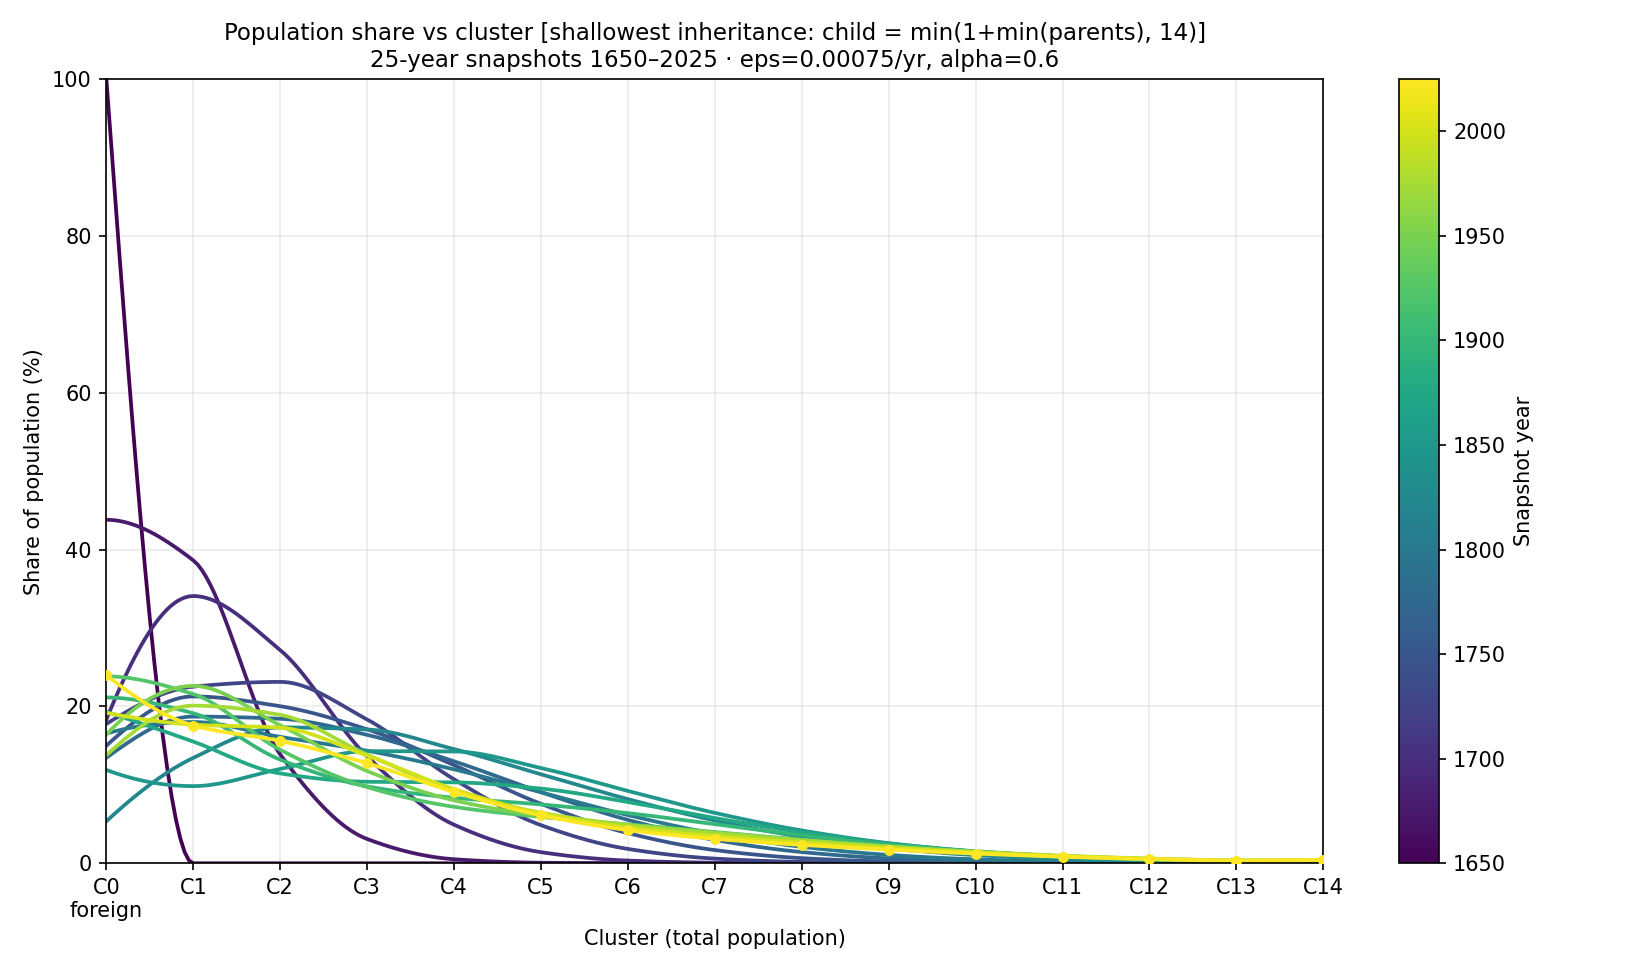
\includegraphics[width=\textwidth]{figs/dist_shallowest_inheritance_linear.png}
  \caption{2025 pedigree-depth distribution under shallowest inheritance,
  two-sex model, $\alpha=0.8$: monotone decline, $C_{14}=0.45\%$.}
  \label{fig:dist-shallow}
\end{figure}
\begin{figure}[htbp]
  \centering
  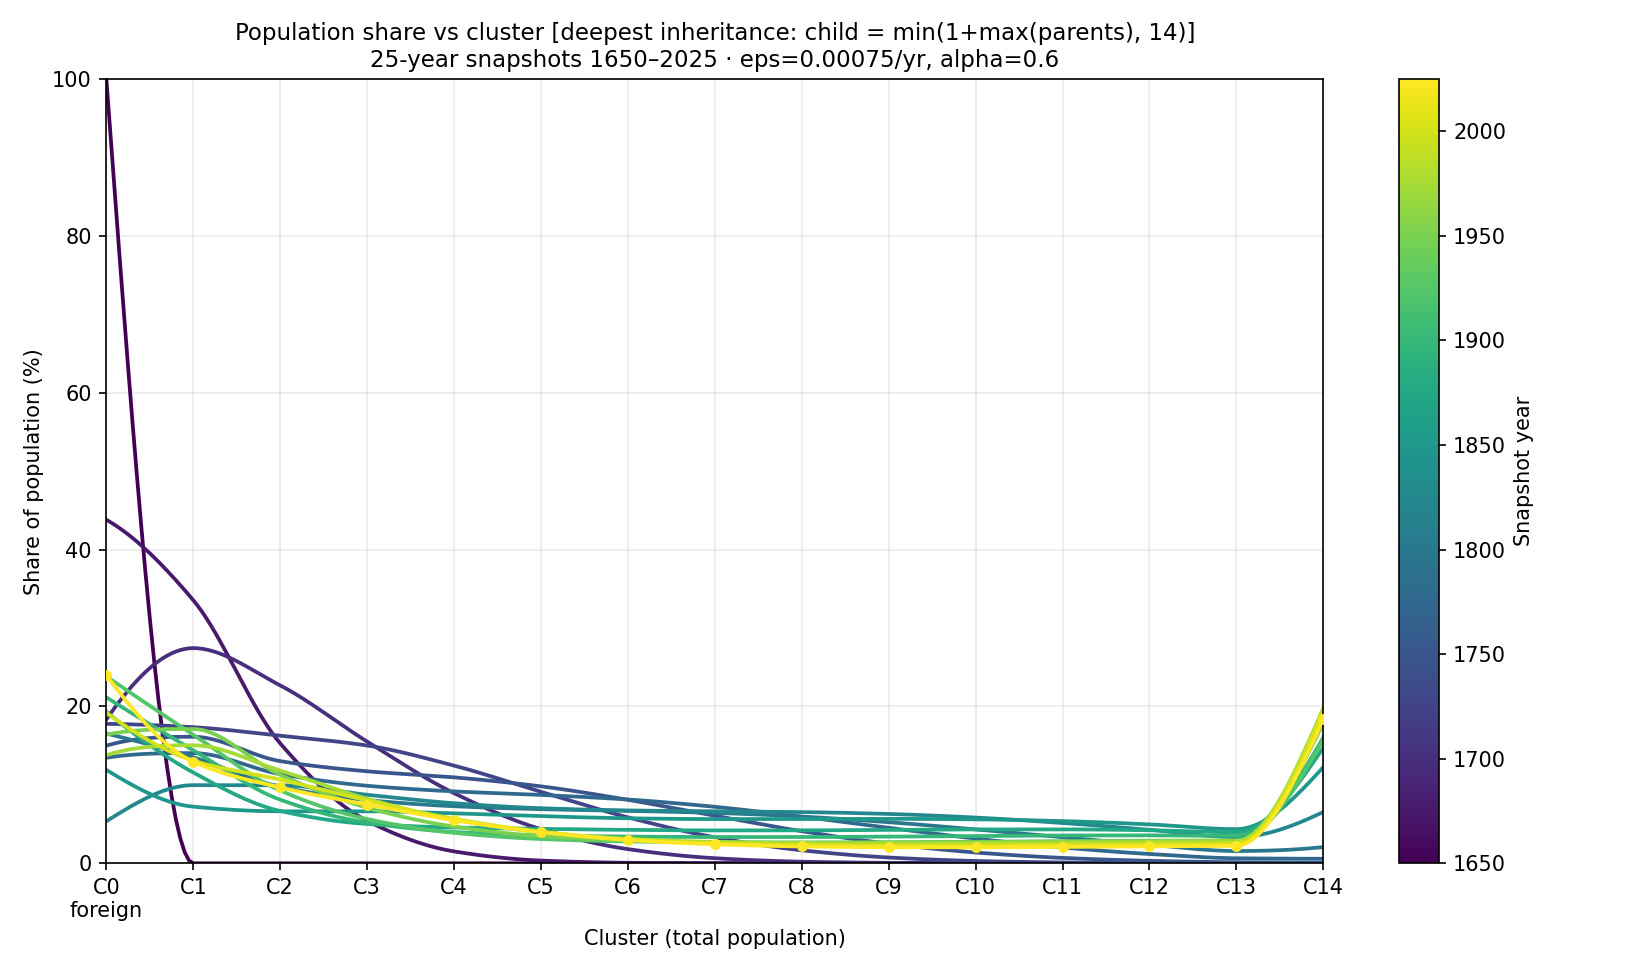
\includegraphics[width=\textwidth]{figs/dist_deepest_inheritance_linear.png}
  \caption{2025 pedigree-depth distribution under deepest inheritance,
  two-sex model, $\alpha=0.8$: the $\sim$2\% plateau across
  $C_8$--$C_{13}$ and the 18.35\% accumulation at the cap $C_{14}$.}
  \label{fig:dist-deep}
\end{figure}

The mechanism is structural.  Under shallowest inheritance, a
deep-by-shallow mating drags the child back to the shallow parent, so
deep mass is constantly recycled downward and only deep-by-deep
pairings sustain it; the distribution falls monotonically and $C_{14}$
holds 0.45\%.  Under deepest inheritance there is no downward pull:
children are always at least as deep as the deeper parent, so every
lineage ratchets upward until it piles at the cap --- $C_{14}$ holds
18.35\%, nearly one in five Americans, with a flat $\sim$2\% plateau
across $C_8$--$C_{13}$ where the ratchet stalls before the final
accumulation.

Assortativity modulates the ratchet but does not remove it.  At
$\alpha=0.0$ (random mating) the deepest rule puts 71.9\% of the
population at the cap, because mixed-depth matings are frequent and
each one steps the lineage up; at $\alpha=0.9$ (strong endogamy) the
cap share falls to 9.4\%, as segregation slows the upward flux.  Under
shallowest inheritance the cap share is 0.00\% at $\alpha=0.0$ and
1.46\% at $\alpha=0.9$.  The qualitative verdict is
$\alpha$-independent: the choice of inheritance rule, not the mating
pattern, decides whether deep pedigree is rare or ubiquitous.

\subsection{Finer scales}
\label{sec:scales}
The same comparison at the finer structural levels confirms the
pattern and reveals one interaction.  In the regional model (four
Census regions, $\alpha=0.8$), 2025 $C_{14}$ is 0.47\% under
shallowest and 18.47\% under deepest inheritance, with the Midwest the
deepest region under both rules.  In the age-structured model the
deepest rule reaches 38.90\% at the cap, against 1.62\% under
shallowest: age structure concentrates deep mass in old cohorts
(the ageless aggregate understates deep clustering 2--4$\times$), and
the deepest rule then ratchets that reservoir to the cap --- the two
effects multiply.

\subsection{Religious dimension}
\label{sec:religious-results}
The eight-group religious model (240 ODEs, $\alpha=0.8$) reproduces the
rule contrast at nearly identical magnitudes: 2025 $C_{14}$ is 0.45\%
under shallowest inheritance and 17.93\% under deepest
inheritance, against two-sex values of 0.45\% and 18.35\%.  The
unaffiliated share reaches 27.9\% in 2025 under both rules --- the
disaffiliation flow is orthogonal to the inheritance rule --- against
Pew's measured 29\% \cite{pew-rls-2025}.  Within-group endogamy
($\rho_g=0.62$--0.87, estimated from Pew surveys) leaves the
between-rule gap intact: long-tenure groups run deep (Protestant
24.5\%, unaffiliated 18.7\% under deepest), while post-1965-immigrant
groups stay shallow (Muslim, Hindu/Buddhist $\approx 1.6\%$); under
shallowest inheritance every group sits below 0.7\%.  The pattern is
demographic, not theological: tenure in the country, not doctrine,
determines depth.

\subsection{Prediction, 2025--2050}
\label{sec:case2}
Case~2 projects 2025--2050 on explicitly projected inputs (vital rates
trend-extrapolated excluding COVID years, immigration fixed at 2024
levels, disaffiliation at its calibrated rate).  The 2050 total is
279.7~million under both rules.  The foreign-born share rises from
24.0\% to 30.2\% --- continued immigration against fixed rates
mechanically dilutes native depth --- while the cap share barely moves:
0.45\% $\to$ 0.42\% (shallowest) and 18.35\% $\to$ 16.66\% (deepest).
The inheritance-rule gap is thus stable over the projection horizon;
demography shifts the distribution's weight toward $C_0$ under either
rule.
% =====================================================================
\section{Conclusions and Future Developments}
% =====================================================================
\label{sec:conclusions}

We have built a forward-time cluster-dynamics model of U.S.\ pedigree
structure, grounded in measured demographic series over 1650--2025 and
projected to 2050, and used it to compare two limiting definitions of
inherited pedigree depth.  Three conclusions stand out.

First, the inheritance rule is the dominant modeling choice.  From
identical births, deaths, immigration, and mating patterns, shallowest
inheritance yields a 2025 America in which 0.45\% of the population
sits in the deepest pedigree cluster, while deepest inheritance yields
18.35\% --- a forty-fold gap produced by pure definition.  Any
empirical claim about ``how deep American roots run'' must therefore
state its inheritance rule, or it is not a claim at all.

Second, the rule's effect is structural, not parametric.  It survives
across assortativity values, across regional and religious
disaggregation, and across the 2025--2050 projection; it is amplified,
not created, by age structure.  Totals are untouched throughout: the
rule redistributes, never creates or destroys, people.

Third, the framework is validated as a forward laboratory.  Hindcast
error is sub-percent on totals, the $\alpha$ calibration is
independently anchored, stochastic ensembles (being regenerated under
the revised rules) test the ODE for finite-population bias,
and the religious projection reproduces Pew's measured unaffiliated
share.  The honest gaps --- the $\sim$24\% total shortfall from
sex-specific mortality and unauthorized accounting, the
Midwest-versus-South deep-geography mismatch against self-reported
ancestry --- are reported as findings, since a model that cannot
disagree with data cannot be trusted where data are absent.

Future developments, in order of priority: (i)~age$\times$religion
joint structure, to test whether the age--deepest interaction found
here concentrates further within high-endogamy groups; (ii)~regional
vital rates and paternal age schedules, replacing the national
schedules currently imposed on every region; (iii)~a settlement-history
process for the colonial spin-up, replacing the all-$C_0$ 1650
approximation; (iv)~re-affiliation flows, now that disaffiliation alone
is calibrated; (v)~coupling the pedigree state to policy scenarios ---
immigration levels, fertility supports --- as a compositional
consequence engine for public policy.

\bibliographystyle{plain}
\bibliography{references}

\end{document}
